\documentclass[EJP,preprint]{ejpecp}
\usepackage{booktabs,array,caption,xcolor,xurl}
\usepackage[shortlabels]{enumitem}
\hypersetup{colorlinks=true,linkcolor=blue!45!black,citecolor=blue!45!black,urlcolor=blue!45!black}
\newcommand{\Z}{\mathbb{Z}}
\newcommand{\E}{\mathbb{E}}
\newcommand{\Prob}{\mathbb{P}}
\newcommand{\Var}{\operatorname{Var}}
\newcommand{\CP}{\mathrm{CP}}
\SHORTTITLE{The bias interval of the elephant random walk}
\TITLE{The bias interval of the elephant random walk}
\hypersetup{pdftitle={The bias interval of the elephant random walk},
pdfauthor={Arjun Pemmasani}}
\AUTHORS{Arjun Pemmasani\footnote{\raggedright Department of Mathematics, Harvey Mudd College,
Claremont, CA 91711, USA. \mbox{\EMAIL{apemmasani@hmc.edu}}\newline
ORCID \href{https://orcid.org/0009-0001-2776-6298}{0009-0001-2776-6298}.}}
\KEYWORDS{elephant random walk; bimodality; shape transition; variation diminution; initial bias}
\AMSSUBJ{60G50}
\AMSSUBJSECONDARY{60F05; 60C05}
\ABSTRACT{Gu\'erin, Laulin, Raschel, and Simon conjectured that the
initial biases giving the superdiffusive elephant random walk a
bimodal limit law form an interval centered at one half, and they
described the problem as challenging. We prove this. For every superdiffusive memory, strongly biased starts are
unimodal, and the limit density has two local maxima exactly when
the bias lies in a proper open interval. Outside it, including
its endpoints, the density has a unique local maximum. The
interval is nonempty exactly above a single memory threshold,
numerically about $0.6688$, whose uniqueness follows from a
positive-weight integral for the central curvature of the
fair-start density. We control sign changes in the finite walk's
first and second differences, including those created at the
boundary, and pass them to the limit. The bias boundary is
continuous and tends to zero at least quadratically fast as memory
tends to one.}
\begin{document}
\raggedbottom
\section{Introduction}\label{sec:intro}\label{sec:notation}

\noindent\begin{minipage}{\linewidth}
\begin{quote}\small\itshape
An elephant and an ant are playing hide and seek. The elephant counts while
the ant hides among many identical anthills, then opens its eyes and knows
at once which one the ant is in. The ant's shoes are outside the door.
\end{quote}
\hfill\textup{(Anonymous)}
\medskip
\end{minipage}

The elephant walk~\cite{schutz2004} has steps $X_i\in\{+1,-1\}$.
Given $X_1,\dots,X_t$, it picks $i$ uniformly from $\{1,\dots,t\}$.
Then $X_{t+1}=X_i$ with probability $1-\varepsilon$, and
$X_{t+1}=-X_i$ otherwise. These choices are independent of each other
and of $X_1$. Put
\[
 A_N=\#\{i\le N:X_i=+1\},\qquad S_N=2A_N-N,\qquad
 P_N(k)=\Prob(A_N=k).
\]
The memory is $a=1-2\varepsilon$ and the initial bias is
$q=\Prob(X_1=1)$. In the original description the copying probability
is $p=(1+a)/2$. After $t$ steps with count $k$, the next step is $+1$
with probability $r_t(k)=\varepsilon+ak/t$. We call $q=1/2$ a fair
start, and $\Prob_+$, $\E_+$ condition on $X_1=1$.

When $a\in(1/2,1)$ the ratio $S_N/N^a$ converges almost surely
\cite{baurbert2016,bercu2018}. Let $h_a$ be the density of the limit
given $X_1=1$. With initial bias $q$ the limit density is
\[
 g_{a,q}(u)=q h_a(u)+(1-q)h_a(-u),\qquad g_a=g_{a,1/2}.
\]
Gu\'erin, Laulin, Raschel, and Simon prove that $h_a$ has one
peak~\cite[Theorem~1.1]{glrs2025}. In~\cite[Remark~2.1(b)]{glrs2025},
they conjecture that $g_{a,q}$ has 2 peaks exactly for $q$ in an open
interval centered at $1/2$, and they describe this problem as
challenging. Our Theorem~\ref{thm:main-limit} answers it with a yes.
Furthermore, our Theorem~\ref{thm:main-analytic} states that the
interval is empty for $a\le a_*$ and nonempty for $a>a_*$, where
$a_*\approx0.6688$.

\subsection{The bias interval and its threshold}\label{sec:results}

\begin{theorem}[the bias interval]\label{thm:main-limit}
For every $a\in(1/2,1)$ there is $b_a\in(0,1/2]$ such that
$g_{a,q}$ has exactly two local maxima if and only if
$b_a<q<1-b_a$. Outside this open interval, including its endpoints,
the density is unimodal with a unique local maximum.
\end{theorem}

In particular $g_{a,q}$ is unimodal for $q\le b_a$ and for
$q\ge1-b_a$. Theorem~\ref{thm:main-analytic} gives the set of $a$ with
$b_a<1/2$.

\begin{theorem}[the analytic threshold]\label{thm:main-analytic}
There is exactly one $a_*\in(2/3,69/100)$ with $g_{a_*}''(0)=0$.
The central curvature is negative below $a_*$ and positive above
it, and $\partial_a g_a''(0)|_{a=a_*}>0$.
The bias interval is empty exactly when $a\le a_*$.
\end{theorem}

Theorem~\ref{thm:main-limit} is Theorems~\ref{thm:two-modes}
and~\ref{thm:biased-limit-modes} together with $b_a>0$ from
Theorem~\ref{thm:bias-continuity}. Theorem~\ref{thm:main-analytic} is
Theorem~\ref{thm:threshold}. These proofs use no computer. The bias
boundary is regular. By Theorem~\ref{thm:bias-continuity}, the function
$a\mapsto b_a$ is continuous on $(1/2,1)$, continuously differentiable
on $(a_*,1)$, and strictly decreasing immediately above $a_*$. By
Corollary~\ref{cor:bias-boundary-rate}, $b_a\to0$ as $a\uparrow1$, and
by Proposition~\ref{prop:quadratic-rate},
$b_a\le82(1-a)^2$ for $a$ close to one. We do not know if $b_a$ is
decreasing on all of $(a_*,1)$ (Section~\ref{sec:open}).

At $a_*$ the fair density has a quartic top
(Lemma~\ref{lem:analytic-quartic}), and the next theorem describes how
the two modes and the bias interval open from it.

\begin{theorem}[the critical exponents]\label{thm:main-critical}
There are positive constants $K_*,Q_*$ such that the positive mode
$\kappa_a$ of $g_a$ and the bias boundary satisfy
\[
 \kappa_a\sim K_*\sqrt{a-a_*},\qquad
 \tfrac12-b_a\sim Q_*(a-a_*)^{3/2}\quad(a\downarrow a_*).
\]
\end{theorem}

The two asymptotics are Propositions~\ref{prop:critical-shape}
and~\ref{prop:bias-cusp}. Theorem~\ref{thm:two-modes} also counts the
inflection points of $g_a$.

\begin{remark}[numerical values]\label{rem:numerics}
Numerically, $a_*\approx0.66881$, $K_*\approx7.2241$, and
$Q_*\approx9.8670$. These values are not used in any proof.
Section~\ref{sec:verify} describes their interval certificates.
\end{remark}

\begin{figure}[t]
\centering
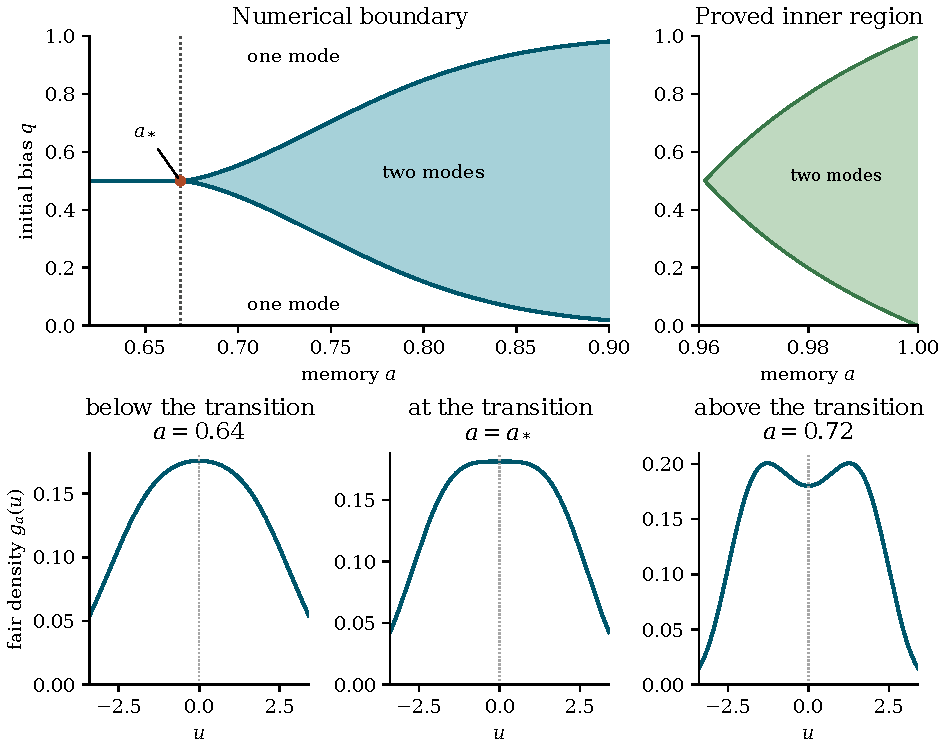
\includegraphics[width=\textwidth]{figures/phase.pdf}
\caption{The bias interval and the fair-start transition. Upper left:
$b_a$ and $1-b_a$ from Theorem~\ref{thm:bias-continuity}, computed
numerically (not certified). Upper right: the region
$4\rho_a/(1-4\rho_a)<q<1-4\rho_a/(1-4\rho_a)$ of
Corollary~\ref{cor:bias-boundary-rate}, which is contained in the
interval. Lower row: $g_a$ for $a=0.64$, $a=a_*$, and $a=0.72$. The top
at $a_*$ is quartic by Lemma~\ref{lem:analytic-quartic}.}
\label{fig:phase}
\end{figure}

\subsection{From finite signs to the limiting shape}\label{sec:architecture}

Gu\'erin, Laulin, Raschel, and Simon prove unimodality by induction on
$N$ for the count law, given $X_1=1$. We do the same induction on every
$q$. By~\eqref{eq:D-rec}, for $2\le k\le t-1$ the value $D_{t+1}(k)$ is
a positive combination of $D_t(k-1)$ and $D_t(k)$. By
Lemma~\ref{lem:interleave}, this step adds no sign change. The new
problem lies at the two ends of a row, because
$D_{t+1}(1)=D_{t+1}(t)=s_{t+1}$ is new, and any value added to the end
can induce a sign change. Hence, we fix the final length $N$ and write
the boundary values $s_N,\dots,s_{t+1}$ entering before time $N$ on
both sides of row $t$. Lemma~\ref{lem:level-one} bounds the signs of
$(s_3,\dots,s_N)$, and then the induction runs over the whole longer
row (Theorem~\ref{thm:five-blocks}). For an arbitrary bias we do the
same with first differences (Figure~\ref{fig:augmented-rows}). By
Proposition~\ref{prop:all-bias-modes}, the first differences within
this longer row swap signs at most 3 times. By
Lemma~\ref{lem:derivative-limits}, all these bounds pass to $g_a$,
$g_a'$, and $g_a''$.

Let $q\ge1/2$. Proposition~\ref{prop:dominant-half} eliminates the
possibility of a $-$ and then a $+$ on the right half. So on
$[0,\infty)$ the density $g_{a,q}$ has no strict valley, and
$g_{a,q}(-x)\le g_{a,q}(x)$. Hence $g_{a,q}$ has two peaks if and only
if $g_{a,q}(x)>g_{a,q}(y)$ for some $x<y\le0$. For fixed $x,y$ this
difference is affine in $q$ and is $\le0$ at $q=1$. If it is positive
at some $q$, it is positive on $[1/2,q]$. Taking the union over $x,y$
and reflecting gives an interval $(b_a,1-b_a)$
(Theorem~\ref{thm:biased-limit-modes}). By
Lemma~\ref{lem:positive-conditional-mode}, $h_a'(0)>0$ for every
$a\in(1/2,1)$, and we can conclude $b_a>0$.

For $a_*$, let $E$ be an independent exponential variable. The
moments of $E^a\mathcal L_a$, where $\mathcal L_a$ is the limit of
$S_N/N^a$ given $X_1=1$, give the transform
of~\cite[Proposition~3.2]{glrs2025}. Two integrations by parts in its Mellin transform give
$g_a''(0)$ as a positive multiple of $\mathcal R(a)-1$, where
$\mathcal R(a)$ is a weighted mean against a positive weight
(Lemma~\ref{lem:curvature-weight}). Rational bounds give the sign of
$g_a''(0)$ for $a\notin[2/3,69/100]$. On $[2/3,69/100]$ the score of
the weight is increasing in the integration variable, and a covariance
identity gives $\mathcal R'(a)>0$
(Appendix~\ref{app:analytic-threshold}). Hence $g_a''(0)$ changes sign
exactly once as $a$ increases (Theorem~\ref{thm:threshold}). The
boundary histories and this positive-weight integral are the new parts
of the argument.

\subsection{Prior work}\label{sec:prior}

The counting chain predates the elephant walk. The Drezner--Farnum
model~\cite{dreznerfarnum1993}, in the formulation of
James, James, and Qi~\cite[p.~2339]{jamesjamesqi2008}, has
next-success probability $(1-\theta)p+\theta k/t$.
With $p=1/2$ and $\theta=a$ this is $r_t(k)$. Their family contains
bimodal laws. Heyde~\cite{heyde2004} gives the limit regimes at fixed
parameters, and James, James, and Qi allow $\theta$ to depend on $t$.
Baur and Bertoin~\cite{baurbert2016} prove functional limit theorems
through P\'olya-type urns. Its memory structure is a random recursive
tree~\cite{kursten2016}, and the split of this tree into two subtrees
is used in Appendix~\ref{app:modes}. Zeros and recurrence of the walk
are studied in~\cite{bertoin2022,qin2025}. See
also~\cite{coletti2017,bercu2018,kubotatakei2019}.

We use the density and moments from~\cite[Theorems~1.3 and~1.4]{glr2026}
and conditional unimodality from~\cite[Theorem~1.1]{glrs2025}. Kiss
and Vet\H{o}~\cite{kissveto2022} compute the first moments for
general steps. Transition probabilities, Gaussian rates, and moment
recurrences are in the preprints
\cite{peresqin2026,muraharatokumitsu2026,vishwakarma2026}.
Trinas and Valle~\cite{tv2026} prove a superdiffusive local limit
theorem, and show the conditional law is not log-concave. Their
difference recurrence also gives Lemma~\ref{lem:derivative-limits}.
Since their paper is a preprint, we include the proof. Trinas~\cite{trinas2026}
uses their local limit theorem for the last-return law, in which the
value $g_{a,q}(0)$ appears.

Da Silva, Cressoni, Sch\"utz, Viswanathan, and
Trimper~\cite{dasilva2013} showed that the superdiffusive propagator is
not Gaussian. In a growing-network model, Mohandas et
al.~\cite[Section~V and Figure~5]{mohandas2025} found the
fair-start transition numerically. They extrapolated finite-$N$
central curvatures and got copying probability about $0.836$. In
their parameter, $a_*$ corresponds to $(1+a_*)/2\approx0.8344$.

The weights giving two peaks are known for normal
mixtures~\cite{eisenberger1964,robertsonfryer1969}, but $h_a$ is not
Gaussian, and the interior step of our induction is classical variation
diminution~\cite{karlin1968,karlin1964}.

\section{Finite shape bounds}\label{sec:convex}

This section proves the finite bounds behind
Theorems~\ref{thm:main-limit} and~\ref{thm:two-modes}. For a fair
start, Theorem~\ref{thm:five-blocks} shows that the second
difference of the count law changes sign at most four times. For
every initial bias, Proposition~\ref{prop:all-bias-modes} shows
that the count law has at most two modal plateaus. The limit
transfer is Lemma~\ref{lem:derivative-limits} in
Appendix~\ref{app:modes}.

We first treat second differences under a fair start. Let
$0<\varepsilon<\frac12$, $a=1-2\varepsilon$, and $r_t(k)=\varepsilon+ak/t$. For $t\ge1$ and every integer $k$ we write
$P_t(k)=\Prob(A_t=k)$, which is $0$ unless $0\le k\le t$, and
\[
 D_t(k)=P_t(k+1)-2P_t(k)+P_t(k-1).
\]
We also put $s_t=D_t(1)=P_t(0)-2P_t(1)+P_t(2)$ for $t\ge2$.

\begin{lemma}[recurrence for the second difference]\label{lem:D-rec}
For every $t\ge1$ and every integer $k$,
\begin{align}
 P_{t+1}(k)&=\bigl(1-r_t(k)\bigr)P_t(k)+r_t(k-1)\,P_t(k-1),\label{eq:P-rec}\\
 D_{t+1}(k)&=\bigl(1-r_t(k+1)\bigr)D_t(k)+r_t(k-2)\,D_t(k-1).\label{eq:D-rec}
\end{align}
Also $P_t(k)=P_t(t-k)$ and $D_t(k)=D_t(t-k)$.
\end{lemma}

\begin{proof}
Given $A_t=k$, the copied step is $+1$ with probability $k/t$, so step $t+1$
is $+1$ with probability $(1-\varepsilon)\frac kt+\varepsilon(1-\frac
kt)=r_t(k)$. This gives \eqref{eq:P-rec} for $0\le k\le t+1$. At $k=0$ and
$k=t+1$, the extra term $r_t(-1)P_t(-1)$ or
$(1-r_t(t+1))P_t(t+1)$ is $0$ because $P_t(-1)=P_t(t+1)=0$.
Outside $0\le k\le t+1$ both sides are $0$.
Under a fair start, $(X_i)$ and $(-X_i)$ have the same law, so
$P_t(k)=P_t(t-k)$. Taking second differences gives the same for $D_t$.

For \eqref{eq:D-rec}, take second differences in \eqref{eq:P-rec}.
The affine identity $r_t(k+1)-r_t(k)=a/t$ gives
\[
 2r_t(k+1)+r_t(k-2)=3r_t(k),\qquad
 r_t(k+1)+2r_t(k-2)=3r_t(k-1),
\]
so the coefficients of $P_t(k)$ and $P_t(k-1)$ agree with the
right side of~\eqref{eq:D-rec}. The outer two coefficients agree directly.
\end{proof}

Trinas and Valle~\cite[(2.2)]{tv2026} use \eqref{eq:P-rec}, the forward equation, for a superdiffusive local
limit theorem. Their higher-difference
recurrence~\cite[(4.10)]{tv2026} is the basis of a computer-certified
study of log-concavity at fixed memory. We use \eqref{eq:D-rec} for a different
purpose, to count sign changes. For $2\le k\le t-1$ its coefficients
are positive. So new changes can only come in at the ends.
Lemma~\ref{lem:interleave} shows that positive sums of neighbors never add a change
(see~\cite{karlin1968,karlin1964} for the general theory).

Let $z$ be a finite real list. Delete its zeros, replace each entry
left by its sign, and merge equal neighbors. What remains is the
sign pattern $\operatorname{sp}(z)$, an alternating list of signs. For
two such lists we write $\sigma\preceq\tau$ if $\sigma$ is a subsequence of $\tau$. We put
$\Pi_5=(+,-,+,-,+)$ and $\Pi_3=(+,-,+)$.

\begin{lemma}[positive sums of neighbors]\label{lem:interleave}
Let $\zeta=(\zeta_1,\dots,\zeta_n)$ be real, and let
$\eta_i=A_i\zeta_i+B_i\zeta_{i+1}$ for $1\le i\le n-1$ with $A_i\ge0$ and
$B_i\ge0$. Let $w=(\zeta_1,\eta_1,\zeta_2,\eta_2,\dots,\eta_{n-1},\zeta_n)$.
Then $\operatorname{sp}(w)=\operatorname{sp}(\zeta)$ and
$\operatorname{sp}(\eta)\preceq\operatorname{sp}(\zeta)$.
\end{lemma}

\begin{proof}
Insert each $\eta_i$ between its two neighbors in $\zeta$. If $\eta_i=0$, the
sign pattern does not change. If $\eta_i>0$, then $\zeta_i>0$ or
$\zeta_{i+1}>0$, so $\eta_i$ is placed next to an entry of its own sign, and
the pattern does not change. The same holds for $\eta_i<0$, proving the first claim.
For the second, obtain $\eta$ from $w$ by deleting the entries
$\zeta_i$. Deletion can only remove signs from the pattern.
\end{proof}

For the walk we apply Lemma~\ref{lem:interleave} to the augmented
rows of Figure~\ref{fig:augmented-rows}, drawn there for first
differences. Proposition~\ref{prop:all-bias-modes} treats the whole
row and Proposition~\ref{prop:dominant-half} the half $2k+1\ge t$.

\begin{figure}[ht]
\centering
\small
\[
\begin{array}{c@{\quad}c@{\quad}c}
\underbrace{\ell_N,\ldots,\ell_{t+1}}_{\text{left boundary history}}&
\underbrace{d_t(0),\ldots,d_t(t-1)}_{\text{active row}}&
\underbrace{u_{t+1},\ldots,u_N}_{\text{right boundary history}}\\[9pt]
&\downarrow\ \text{copy or sum adjacent entries}&\\[9pt]
\ell_N,\ldots,\ell_{t+2}&
\ell_{t+1},d_{t+1}(1),\ldots,d_{t+1}(t-1),u_{t+1}&
u_{t+2},\ldots,u_N
\end{array}
\]
\caption{One step of the augmented rows for a final length $N$, with
$d_t(k)=P_t(k+1)-P_t(k)$, $\ell_t=d_t(0)$, and $u_t=d_t(t-1)$. The
active row gains an entry and the histories on each side lose one.
Each new end value was already in a history, so the bound for the
previous row already counts its sign.}
\label{fig:augmented-rows}
\end{figure}

\begin{lemma}[sign changes next to an end]\label{lem:level-one}
For every $t_1\ge2$ we have $\operatorname{sp}(s_2,s_3,\dots,s_{t_1})\preceq\Pi_3$.
\end{lemma}

We prove this in Appendix~\ref{app:signs-level}.

\begin{theorem}[at most five blocks]\label{thm:five-blocks}
Let $N\ge3$ and $0<\varepsilon<\frac12$. Then
\[
 \operatorname{sp}\bigl(D_N(1),D_N(2),\dots,D_N(N-1)\bigr)\preceq(+,-,+,-,+).
\]
So the second difference of $P_N$ changes sign at most four times on
$\{1,\dots,N-1\}$.
\end{theorem}

\begin{proof}
For $3\le t\le N$, we retain the endpoint history in the list $\mathcal Z_t$
\[
 \mathcal Z_t=\bigl(s_N,s_{N-1},\dots,s_{t+1},\ s_t,D_t(2),D_t(3),\dots,D_t(t-2),s_t,\
 s_{t+1},\dots,s_{N-1},s_N\bigr).
\]
It has $2N-t-1$ entries. Its middle part is
$(D_t(1),D_t(2),\dots,D_t(t-1))$, because $D_t(t-1)=D_t(1)=s_t$ by symmetry.
The list $\mathcal Z_3$ is $(s_N,\dots,s_4,s_3,s_3,s_4,\dots,s_N)$, and $\mathcal Z_N$ is the
list in the statement.

To apply Lemma~\ref{lem:interleave}, we check how
$\mathcal Z_{t+1}$ is obtained from $\mathcal Z_t$ for $3\le t\le N-1$. The first $N-t$ entries of
$\mathcal Z_{t+1}$ are $s_N,\dots,s_{t+1}$, and they are copies of the first $N-t$
entries of $\mathcal Z_t$. So $A_i=1$ and $B_i=0$ there. The next $t-2$ entries are
$D_{t+1}(j)$ for $2\le j\le t-1$. By \eqref{eq:D-rec},
\[
 D_{t+1}(j)=r_t(j-2)\,D_t(j-1)+\bigl(1-r_t(j+1)\bigr)D_t(j),
\]
and $D_t(j-1)$ and $D_t(j)$ are neighbors in the middle part of $\mathcal Z_t$, in the
required order. The coefficients satisfy $r_t(j-2)\ge\varepsilon$ and
$1-r_t(j+1)\ge1-\varepsilon-a=\varepsilon$, since $2\le j\le t-1$. The last
$N-t$ entries of $\mathcal Z_{t+1}$ are $s_{t+1},\dots,s_N$, and each is a copy of the
entry of $\mathcal Z_t$ one place to its right. So $A_i=0$ and $B_i=1$ there.

By Lemma~\ref{lem:interleave},
$\operatorname{sp}(\mathcal Z_N)\preceq\operatorname{sp}(\mathcal Z_{N-1})\preceq\dots\preceq\operatorname{sp}(\mathcal Z_3)$.
By Lemma~\ref{lem:level-one} the sign pattern $p$ of $(s_3,\dots,s_N)$ is a
subsequence of $\Pi_3$, so it is one of the lists $()$, $(+)$, $(-)$, $(+,-)$,
$(-,+)$, and $(+,-,+)$. The sign pattern of $\mathcal Z_3$ is $p$ reversed, followed by
$p$, with equal neighbors merged. In the six cases this is $()$, $(+)$, $(-)$,
$(-,+,-)$, $(+,-,+)$, and $(+,-,+,-,+)$, and each is a subsequence of $\Pi_5$.
\end{proof}

\subsection{First differences for a biased start}\label{sec:biased-finite}

\begin{proposition}[two modes for every initial bias]\label{prop:all-bias-modes}
Let $0<\varepsilon<1$, let $q\in[0,1]$ be the probability that the first
step is positive, and let $P_n(k)$ be the law of the number of positive
steps after $n\ge1$ steps. Extend $P_n$ by zero outside $\{0,\ldots,n\}$.
The first differences $d_n(k)=P_n(k+1)-P_n(k)$ satisfy
\[
 \operatorname{sp}\bigl(d_n(-1),d_n(0),\ldots,d_n(n)\bigr)
 \preceq (+,-,+,-).
\]
In particular, $P_n$ has at most two modal plateaus, including endpoint
modes. Moreover, there are no integers $i_0<\cdots<i_4$ for which
\[
 P_n(i_0)>P_n(i_1)<P_n(i_2)>P_n(i_3)<P_n(i_4).
\]
\end{proposition}

\begin{proof}
Put $a=1-2\varepsilon$ and $r_t(k)=\varepsilon+ak/t$. The forward equation
is
\[
 P_{t+1}(k)=(1-r_t(k))P_t(k)+r_t(k-1)P_t(k-1),
 \qquad P_1=(1-q,q).
\]
Subtracting adjacent equations gives
\begin{equation}\label{eq:bias-first-diff}
 d_{t+1}(k)=r_t(k-1)d_t(k-1)+(1-r_t(k+1))d_t(k),
 \qquad 1\le k\le t-1.
\end{equation}
Both coefficients are at least $\min(\varepsilon,1-\varepsilon)>0$,
since $r_t(j)$ is a convex combination of $\varepsilon$ and
$1-\varepsilon$ for $0\le j\le t$. It remains to check the two ends.

Suppose first that $q<1$. Since
$P_t(0)=(1-q)(1-\varepsilon)^{t-1}>0$, define
\[
 \xi_t=\frac{P_t(1)}{P_t(0)},\qquad
 b=\frac{1-2\varepsilon}{1-\varepsilon}<1,\qquad
 A=\frac{\varepsilon}{1-\varepsilon}>0.
\]
The boundary equation gives
\[
 \xi_{t+1}=(1-b/t)\xi_t+A,\qquad \xi_1=\frac q{1-q}.
\]
Thus $\delta_t=\xi_{t+1}-\xi_t$ obeys
\begin{equation}\label{eq:bias-edge-increments}
 \delta_{t+1}=\frac{t-b}{t+1}\delta_t+\frac A{t+1}.
\end{equation}
Once an increment is nonnegative, every later increment is positive.
Thus $\xi_t$ first decreases and then increases (either part may be empty). For $\ell_t=d_t(0)=P_t(0)(\xi_t-1)$ this proves
\[
 \operatorname{sp}(\ell_1,\ldots,\ell_N)\preceq(+,-,+).
\]
If $q\le1/2$, then $\xi_1\le1$ and the sharper bound is
$\operatorname{sp}(\ell_1,\ldots,\ell_N)\preceq(-,+)$.
In particular, a positive $\ell_i$ cannot be followed by a negative
$\ell_j$. Zeros do not affect either conclusion.

Write $u_t=d_t(t-1)$. Reflection of the walk gives
$u_t(q)=-\ell_t(1-q)$ and
$d_t^{(1-q)}(t-1-k)=-d_t^{(q)}(k)$.
For $0<q\le1/2$, the right boundary history therefore has pattern
contained in $(-,+,-)$. For $q=0$ it is nonpositive throughout. The conditional count is at
most $t-1$, so $u_t=-P_t(t-1)\le0$.

We put the values arriving at the boundary in an augmented row, since
they are not controlled by the interior recurrence. Fix $N$ and, for
$1\le t\le N$, form
\[
 Z_t=(\ell_N,\ldots,\ell_{t+1},
       d_t(0),\ldots,d_t(t-1),
       u_{t+1},\ldots,u_N).
\]
The left history is read backwards while the right is read forwards,
so every endpoint that arrives was already in the previous augmented
row and the recurrence ends up controlling the entire row.
For $q\le1/2$, its first row is contained in $(+,-,+,-)$.
We must also allow zeros at $\ell_1=u_1=2q-1$. Suppose $Z_1$
contained four ordered signs $-,+,-,+$. If the second lay in the
reversed left history, the first two would give
a positive left edge followed in time by a negative one, which is
impossible. Otherwise the last three lie in the right history and have
signs $+,-,+$. For $q>0$, their reflected negatives give the forbidden pattern
$(-,+,-)$ in the left history at bias $1-q$. For $q=0$, they contradict
the nonpositive right history. This also covers $N=1$.

Every entry of $Z_{t+1}$ is a nonnegative combination of adjacent entries
of $Z_t$. The interior entries use \eqref{eq:bias-first-diff}. The two new
boundary entries and the remaining future edge values are copied,
with coefficients $(1,0)$ or $(0,1)$. To check the ordering, number the augmented entries from left to
right. Output entry $i$ uses input entries $i$ and $i+1$, with a zero
coefficient when copied. A nonzero output
has a parent of the same sign. Two neighbors in the subsequence with
opposite signs cannot share a parent, since one entry has only one
sign. So the parent indices strictly increase. Pick parents like this
for an alternating subsequence of the output. We get the same signs,
in the same order, in the input.
An update therefore cannot add an alternating pattern, so
$\operatorname{sp}(Z_N)\preceq(+,-,+,-)$. Reflection and sign
reversal preserve this pattern, proving the claim also for $q\ge1/2$,
including $q=1$.

Finally, extension by zero adds $d_N(-1)=P_N(0)\ge0$ on the left and $d_N(N)=-P_N(N)\le0$ on the right. Neither enlarges the pattern.
Every modal plateau contributes a positive-to-negative change, so there
are at most two. If the statement's last inequalities held, telescoping
on each of their four intervals would give an adjacent difference
of the same strict sign. These four differences would
have signs $-,+,-,+$, a contradiction.
\end{proof}

\section{The limit density at fixed memory}\label{sec:bulk-applications}

Fix $\varepsilon\in(0,\frac14)$, so $a=1-2\varepsilon\in(\frac12,1)$.
Conditional on $X_1=1$, $S_k/k^a$ converges almost surely to
$\mathcal L_a$~\cite[Theorem~3.7]{bercu2018}. The fair-start limit
$\mathcal L^\circ_a$ has the law of $\xi\mathcal L_a$, where $\xi$ is a fair sign independent of
$\mathcal L_a$~\cite[(1.3) and (1.6)]{glr2026}. Gu\'erin, Laulin, and Raschel
prove that both limits have positive, bounded, and smooth
densities~\cite[Theorem~1.3]{glr2026}, denoted by $h_a$ and $g_a$ as before.
Gu\'erin, Laulin, Raschel, and Simon prove
that $\mathcal L_a$ is unimodal~\cite[Theorem~1.1]{glrs2025}.
We also use two regularity facts, proved in
Lemma~\ref{lem:analytic-density} of Appendix~\ref{app:regularity}. For
every bias $q$, the limit density extends to an entire function, so it
is not constant on any interval. For every $k\ge0$, the derivatives
$\partial_u^k h_a(u)$ and $\partial_a\partial_u^k h_a(u)$ exist and are
jointly continuous in $(a,u)$.

\subsection{Modes and inflection points}\label{sec:modes}

A probability density $h$ on $\mathbb R$ is \emph{unimodal} if for some $m$
it is nondecreasing on $(-\infty,m]$ and nonincreasing on $[m,\infty)$.
Gu\'erin, Laulin, Raschel, and Simon ask for a unique local maximum~\cite{glrs2025},
so we must also exclude a flat top. The density $g_a$ mixes the
unimodal density of $\mathcal L_a$ with its reflection. Such a
mixture can have more than one peak~\cite{dj1988}. We first take a fair start.
Lemma~\ref{lem:analytic-density} excludes constant intervals,
so modes are points. We consider other biases afterward.

\begin{theorem}[at most two modes]\label{thm:two-modes}
Let $a\in(\frac12,1)$. Exactly one of the following holds.
\begin{enumerate}[(a)]
\item The density $g_a$ is nondecreasing on $(-\infty,0]$ and nonincreasing on
$[0,\infty)$.
\item There is $\kappa>0$ such that $g_a$ is nondecreasing on $[0,\kappa]$ and
nonincreasing on $[\kappa,\infty)$, and $g_a(0)<g_a(\kappa)$.
\end{enumerate}
In case (b), $g_a$ is nondecreasing on $(-\infty,-\kappa]$ and nonincreasing on
$[-\kappa,0]$, and it is not unimodal. All these monotonicities are strict.
The unique local maximum is $0$ in case (a), and the only local maxima
are $\pm \kappa$ in case (b).
In case (a), there is $d>0$ such that $g_a$ is strictly concave on
$(-d,d)$ and strictly convex on each tail. In case (b), there are
$0<d_1<\kappa<d_2$ such that $g_a$ is strictly convex on $(-d_1,d_1)$ and
on each tail beyond $\pm d_2$, and strictly concave on
$(-d_2,-d_1)$ and $(d_1,d_2)$. Thus it has exactly two inflection points
in case (a) and four in case (b).
\end{theorem}

A real function $v$ has \emph{values at most} $\Pi$ if
$\operatorname{sp}(v(y_1),\ldots,v(y_j))\preceq\Pi$ for every
$y_1<\cdots<y_j$.

\begin{proof}
Fix $a\in(1/2,1)$. Lemma~\ref{lem:derivative-limits} at order two
passes the five-block bound of Theorem~\ref{thm:five-blocks} to
$g_a''$. Indeed, the interpolant's values are positive sums of
adjacent second differences, and its lattice fills every fixed
compact interval as $N\to\infty$. Lemmas~\ref{lem:interleave}
and~\ref{lem:sp-limit} therefore give values at most $\Pi_5$.


\emph{Symmetry.} Proposition~\ref{prop:dominant-half} and
Lemma~\ref{lem:derivative-limits}, with $r=0$, show that $g_a$
has no strict valley on $[0,\infty)$. Such a valley would persist
at nearby lattice points under locally uniform convergence.

If every increment on $[0,\infty)$ is nonpositive, case (a)
holds. Otherwise choose $y_1<y_2$ with $g_a(y_1)<g_a(y_2)$.
Integrability supplies $y_3<y_4$, both beyond $y_2$, with
$g_a(y_3)>g_a(y_4)$. The no-valley property excludes any later increase,
so $g_a$ attains a maximum on $[0,\infty)$ at some $\kappa$.
The absence of a strict valley makes it nondecreasing before
$\kappa$ and nonincreasing afterward. The positive increment forces
$\kappa>0$. If $g_a(0)=g_a(\kappa)$,
it would be constant on $[0,\kappa]$, contrary to analyticity
and the positive increment. Thus case (b) holds.
Evenness gives the left-half shape and excludes unimodality in (b).

Equality at two points of a monotone interval would force a constant
interval, contrary to Lemma~\ref{lem:analytic-density}. Thus the
monotonicities are strict and there is no additional local maximum.

\emph{Curvature.} The Fourier bound in
Lemma~\ref{lem:analytic-density} gives $g_a(y),g_a'(y)\to0$ as
$y\to\infty$. Evenness and the $\Pi_5$ bound give at most three sign
blocks for $g_a''$ on $(0,\infty)$. Its last sign must be positive. Otherwise $g_a'$ would eventually
be nonincreasing with limit zero, making $g_a$ eventually nondecreasing.
This contradicts $g_a>0$ and $g_a\to0$.
Analyticity and strict monotonicity imply that the first nonconstant
term in the even Taylor series of $g_a$ at zero is negative in case (a)
and positive in case (b). The same signs therefore hold for $g_a''$
near zero. In case (b), $g_a''$ must also be negative somewhere, since
$g_a'$ is positive near zero and negative somewhere beyond $\kappa$.
The positive-half-line sign patterns are consequently $(-,+)$ in
case (a) and $(+,-,+)$ in case (b). Analyticity excludes an interval
of zero curvature and makes the resulting convexities strict. In
case (b), $g_a'(d_1)>0>g_a'(d_2)$, so $d_1<\kappa<d_2$.
\end{proof}

\begin{theorem}[the unique transition]\label{thm:threshold}
There is exactly one $a_*\in(1/2,1)$ with $g_{a_*}''(0)=0$.
It lies in $(2/3,69/100)$, and
\[
 g_a''(0)<0\quad(1/2<a<a_*),\qquad
 g_a''(0)>0\quad(a_*<a<1).
\]
Moreover, $\partial_a g_a''(0)|_{a=a_*}>0$.
The density $g_a$ is unimodal for $a\le a_*$ and bimodal for
$a>a_*$. In particular, the critical density is unimodal.
\end{theorem}

To rule out a second crossing, Appendix~\ref{app:analytic-threshold}
expresses the curvature sign as a comparison of positive weighted
means, without numerical input. Rational bounds fix the sign outside
$[2/3,69/100]$. On this interval the score is increasing, and a
covariance identity shows that the weighted mean is strictly
increasing in $a$. Hence there is exactly one crossing.
Numerically $a_*\approx0.66881$ (Remark~\ref{rem:numerics}).

\subsection{Arbitrary initial bias}

Write $h_a$ for the density of $\mathcal L_a$ and
$g_{a,q}(x)=q h_a(x)+(1-q)h_a(-x)$ for initial bias
$\Prob(X_1=1)=q$. Thus $g_{a,1/2}=g_a$.

\begin{theorem}[the interval of bimodal biases]\label{thm:biased-limit-modes}
For every $a\in(1/2,1)$ and $q\in[0,1]$, the density $g_{a,q}$ has at
most two local maxima. There is $b_a\in(0,1/2]$ such that it has exactly
two local maxima if and only if
\[
                 b_a<q<1-b_a.
\]
Outside this open interval, including its endpoints, the density is
unimodal with a unique local maximum. The interval is empty exactly when
$a\le a_*$, in which case $b_a=1/2$. Positivity of $b_a$ for
$a>a_*$ is proved in Theorem~\ref{thm:bias-continuity}.
At finite time, for every $0<\varepsilon<1$, $q\in[0,1]$, and
$N\ge1$, the count law has at most two modal plateaus, including its
endpoints.
\end{theorem}

\begin{proof}
\emph{The mode bound.} Proposition~\ref{prop:all-bias-modes}
gives the finite assertion and excludes two successive strict valleys.
The locally uniform density convergence in
Lemma~\ref{lem:derivative-limits}, with $r=0$, passes these
inequalities to $g_{a,q}$.
Lemma~\ref{lem:analytic-density} excludes constant intervals
for every bias. Hence three local maxima $x<y<z$
would give
$x<u<y<v<z$ with
\[
 g_{a,q}(u)<\min\{g_{a,q}(x),g_{a,q}(y)\},\qquad
 g_{a,q}(v)<\min\{g_{a,q}(y),g_{a,q}(z)\}.
\]
For each pair, take a one-sided neighborhood of the smaller maximum
toward the other one. Since the density is not constant on an
interval, some point there has strictly smaller value. This gives
the two forbidden valleys.

\emph{The bias interval.} Fix $a$, write $f_q=g_{a,q}$ and $h=h_a$,
and call $x<y<z$ a strict valley if $f_q(y)<\min\{f_q(x),f_q(z)\}$.
Proposition~\ref{prop:dominant-half} and the same density convergence show that,
for $q\ge1/2$, $f_q$ has no strict valley on $[0,\infty)$ and
$f_q(-x)\le f_q(x)$ for $x\ge0$.
Thus it has a strict valley if and only if
$f_q(x)>f_q(y)$ for some $x<y\le0$. Reflection dominance turns
such a descent into the valley $(x,y,-x)$. Conversely, a valley
must start at $x<0$. If its middle point $y$ is positive,
the no-valley property at $(0,y,z)$ gives
$f_q(0)\le f_q(y)<f_q(x)$.

At $q=1$, conditional unimodality~\cite{glrs2025} and reflection
dominance place the mode in $[0,\infty)$. A negative mode would have
a reflected point of at least the same height, contrary to uniqueness.
Thus $h$ is nondecreasing on $(-\infty,0]$. For fixed $x<y\le0$, the
difference $f_q(x)-f_q(y)$ is affine in $q$ and nonpositive at $q=1$.
If positive at $q\ge1/2$, it remains positive for every $q'\in[1/2,q]$.
Thus, within $[1/2,1]$, a valley persists when the bias decreases.
These biases form a relatively open set because the strict
inequalities at three fixed points survive a small change of bias.
The set excludes $1$, and reflection gives an open interval
$(b_a,1-b_a)$, possibly empty.

A strict valley gives two local maxima. Integrability and positivity
let us choose an outer point on each side below the corresponding
high point. We then maximize on the two resulting compact
intervals. Conversely, two local
maxima give a strict valley because there is no flat interval.
The mode bound excludes a third maximum. A continuous integrable
density without a strict valley is unimodal, and absence of flat
intervals makes its maximum unique. Finally the bias interval is
nonempty exactly when it contains $1/2$, so
Theorem~\ref{thm:threshold} identifies the empty case.
\end{proof}

This proves the initial-bias conjecture
of~\cite[Remark~2.1(b)]{glrs2025}, with its half-width $q(a)=1/2-b_a$.
The derivative-limit argument used here is proved in Appendix~\ref{app:modes}.

\subsection{The bias boundary}

For $a>a_*$, Theorem~\ref{thm:threshold} puts $g_a$ in case (b) of
Theorem~\ref{thm:two-modes}. We write $\kappa_a$ for its positive
mode $\kappa$.

To find the endpoint, we compare the conditional density's slopes
at reflected points. Their ratio tells us how much weight the
reflected density needs to create a decrease.

\begin{proposition}[a variational equation for the bias boundary]
\label{prop:bias-boundary}
For $a\in(1/2,1)$ put $U_a=\{t>0:h_a'(t)>0\}$. With the infimum
over an empty set interpreted as $+\infty$,
\begin{equation}\label{eq:bias-boundary}
 b_a=\min\left\{\frac12,\quad
       \inf_{t\in U_a}\frac{h_a'(-t)}{h_a'(t)+h_a'(-t)}\right\}.
\end{equation}
If the infimum is attained
at $t>0$ with $h_a'(t)>0$ and $b_a<1/2$, then, with $q=1-b_a$,
\[
 g_{a,q}'(-t)=g_{a,q}''(-t)=0.
\]
At this point the smaller peak disappears.
\end{proposition}

\begin{proof}
The proof of Theorem~\ref{thm:biased-limit-modes} shows that
$h_a'(-t)\ge0$ for $t\ge0$. For $q\ge1/2$ bimodality is equivalent
to a decrease somewhere on the negative half-line, hence to
$g_{a,q}'(-t)<0$ for some $t>0$. Here
\[
 g_{a,q}'(-t)=q h_a'(-t)-(1-q)h_a'(t).
\]
This expression can be negative only if $t\in U_a$, in which case
it is negative exactly when
$1-q>h_a'(-t)/(h_a'(t)+h_a'(-t))$. Taking the union over $t$ gives
\eqref{eq:bias-boundary}, with equality excluded as in
Theorem~\ref{thm:biased-limit-modes}. At an interior minimizer the
ratio has derivative zero. Differentiating its numerator and
denominator gives the two displayed equations.
\end{proof}

\begin{theorem}[regularity of the bias boundary]\label{thm:bias-continuity}
The function $a\mapsto b_a$ is continuous on $(1/2,1)$, is continuously
differentiable on $(a_*,1)$, and extends continuously to $b_1=0$.
It is strictly decreasing on some interval immediately above $a_*$.
For every $a>a_*$, we have $0<b_a<1/2$,
and the infimum in
\eqref{eq:bias-boundary} has a unique minimizer $t_a\in(0,\kappa_a)$.
This minimizer depends continuously on $a$ throughout $(a_*,1)$.
\end{theorem}

\begin{proof}
For $a>a_*$, the curvature partition in Theorem~\ref{thm:two-modes}
gives $g_a'(t)>0$ on $(0,\kappa_a)$ and $g_a'(t)<0$ on
$(\kappa_a,\infty)$. For $t\ge\kappa_a$ in $U_a$, the ratio in
\eqref{eq:bias-boundary} is therefore at least $1/2$.
Since $b_a<1/2$, it is enough to search $(0,\kappa_a)$
(we still have to show the infimum is attained).
Put
\[
 D_a(t)=h_a'(t)+h_a'(-t),\qquad
 R_a(t)=\frac{g_a'(t)}{D_a(t)}\quad(0<t<\kappa_a).
\]
Lemmas~\ref{lem:balanced-start} and~\ref{lem:positive-conditional-mode}
give $h_a'(-t)>0$ for every $t\ge0$.
We therefore have $D_a>0$, $0<R_a<1/2$, and
$1/2-b_a=\sup_{0<t<\kappa_a}R_a(t)$. Also $R_a(0+)=0$.

We first rule out a strict valley in the ratio. We claim that
\begin{equation}\label{eq:bias-quasiconcave}
 R_a(v)\ge\min\{R_a(u),R_a(w)\}
 \qquad(0<u<v<w<\kappa_a).
\end{equation}
Otherwise, choose $s\in(0,1/2)$ strictly between the middle value
and both outer values. With $q=1/2+s$,
$g_{a,q}'(-t)=D_a(t)(s-R_a(t))$ then has signs $-,+,-$
at $-w,-v,-u$, and is positive sufficiently close to zero on the left.
Positivity of the density
and its zero limits at infinity supply a positive derivative farther
left and a negative derivative farther right. There would be three
local maxima, contrary to Theorem~\ref{thm:biased-limit-modes}.

At $\kappa_a$, we have $D_a(\kappa_a)=2h_a'(-\kappa_a)>0$.
Thus $R_a$ extends continuously to $[0,\kappa_a]$, with value
zero at both endpoints. Its positive maximum is attained in the
interior. At that point $h_a'(-t)>0$, so the maximum is strictly
below $1/2$. Hence $b_a>0$. We need attainment here (pointwise strict
inequality on an open interval would not suffice).
Equation~\eqref{eq:bias-quasiconcave} and analyticity make this
maximum unique, since two maximizers would force a constant interval.
They also make $R_a$ strictly increasing before its maximizer and
strictly decreasing after it.

Lemma~\ref{lem:analytic-density} gives joint continuity of all the
derivatives used here. The signs of $g_a'$ on either side of its
unique positive zero give continuity of $\kappa_a$. Fix $a_0>a_*$
and choose
$0<l<t_{a_0}<r<\kappa_{a_0}$. The strict inequalities
$R_a(l),R_a(r)<R_a(t_{a_0})$ persist near $a_0$.
For $v<l$, apply \eqref{eq:bias-quasiconcave} to
$v,l,t_{a_0}$. Since $R_a(l)<R_a(t_{a_0})$, it gives
$R_a(v)\le R_a(l)$. Applying it to $t_{a_0},r,v$ gives
$R_a(v)\le R_a(r)$ for $v>r$.
Thus every nearby global maximum lies in the fixed interval $[l,r]$.
The ratios converge uniformly on this fixed compact interval,
so their maxima converge. Uniqueness gives convergence of the
maximizers too. This proves continuity above $a_*$.

At $a_*$, the curvature partition in Theorem~\ref{thm:two-modes}(a)
makes $g_{a_*}'$ strictly decrease from zero and then strictly increase
to zero. Thus $g_{a_*}'(r)<0$ for every $r>0$.
Joint continuity gives $g_a'(r)<0$ for all $a>a_*$ sufficiently close
to $a_*$, so $\kappa_a<r$. Since $r$ was arbitrary, $\kappa_a\to0$.
On the shrinking interval $[0,\kappa_a]$, joint continuity now gives
\[
 \sup_{0\le t\le\kappa_a}|g_a'(t)|\longrightarrow0,\qquad
 \inf_{0\le t\le\kappa_a}D_a(t)\longrightarrow2h_{a_*}'(0)>0,
\]
where the strict inequality is Lemma~\ref{lem:positive-conditional-mode}.
Consequently $1/2-b_a=\max R_a\to0$. Below the threshold $b_a=1/2$,
so this proves continuity at $a_*$ without the critical expansion.
Corollary~\ref{cor:bias-boundary-rate} gives the limit at one.

For differentiability, the same three-point argument puts all nearby
maximizers in one compact interval. If $M(a)=1/2-b_a$, maximality gives,
for $s>0$,
\[
 R_{a+s}(t_a)-R_a(t_a)
 \le M(a+s)-M(a)
 \le R_{a+s}(t_{a+s})-R_a(t_{a+s}).
\]
Divide by $s$ and use the continuity of $t_a$ and
$\partial_aR_a$ from Lemma~\ref{lem:analytic-density}. The argument
for $s<0$ is the same. Thus
\begin{equation}\label{eq:bias-envelope-derivative}
 -b_a'=
 \frac{\partial_a h_a'(t_a)\,h_a'(-t_a)
       -h_a'(t_a)\,\partial_a h_a'(-t_a)}
      {\{h_a'(t_a)+h_a'(-t_a)\}^2}.
\end{equation}
The right side is continuous. No derivative of $t_a$ is needed.

Finally, put $C_*=\partial_a g_a''(0)|_{a=a_*}>0$ and
$H_*=h_{a_*}'(0)>0$, by Theorem~\ref{thm:threshold} and
Lemma~\ref{lem:positive-conditional-mode}.
Extend $R_a=g_a'/D_a$ to a fixed neighborhood of zero, where
$D_a>0$ for $a$ close to $a_*$. Evenness and
Lemma~\ref{lem:analytic-density} give, jointly as $(a,t)\to(a_*,0)$,
\[
 g_a'(t)=o(t),\qquad \partial_a g_a'(t)=(C_*+o(1))t,\qquad
 D_a(t)=2H_*+o(1),\qquad \partial_aD_a(t)=O(1).
\]
For the first two relations, integrate $g_a''$ and $\partial_a g_a''$
from zero to $t$, using $g_{a_*}''(0)=0$.
It follows that
\[
 \partial_aR_a(t)=\left(\frac{C_*}{2H_*}+o(1)\right)t>0
\]
for all sufficiently small $t>0$ and $a$ sufficiently close to $a_*$.
Since $0<t_a<\kappa_a\to0$, the envelope formula gives $b_a'<0$
on some interval immediately above the threshold.
\end{proof}

\begin{corollary}[a rate for the bias boundary near one]\label{cor:bias-boundary-rate}
Put
\[
 \rho_a=\frac{\Gamma(1+a)^2}{(2a-1)\Gamma(2a)}-1.
\]
If $\rho_a<1/12$, then
\[
 b_a\le\frac{4\rho_a}{1-4\rho_a}.
\]
In particular, as $a\uparrow1$,
$b_a\le8(1-a)+O((1-a)^2)$.
\end{corollary}

\begin{proof}
The conditional limit has mean $\mu_a=1/\Gamma(1+a)>0$ and variance
$\rho_a\mu_a^2$, by the moment formulas of~\cite[Theorem~1.4]{glr2026}.
Consider the three adjacent intervals of length $\mu_a$ centered at
$-\mu_a$, $0$, and $\mu_a$. Chebyshev's inequality puts at least
$1-4\rho_a$ of the conditional law in the right interval and at most
$4\rho_a$ in the middle. For a start to the left, reflect these
intervals. After mixing, the left interval has mass at least
$(1-q)(1-4\rho_a)$ and the right at least $q(1-4\rho_a)$.
The middle still has mass at most $4\rho_a$.

For $4\rho_a/(1-4\rho_a)<q<1-4\rho_a/(1-4\rho_a)$, the middle
has less mass than either outer interval. All three intervals have
the same length. So, by continuity, we can choose a point in each
with the middle value strictly smaller than the other two.
This rules out unimodality. The two-mode bound in
Theorem~\ref{thm:biased-limit-modes} gives exactly two modes, and
therefore the stated bound on $b_a$. Finally, the logarithmic derivative at $a=1$
of $1+\rho_a$ is $2\psi(2)-2-2\psi(2)=-2$.
Thus $\rho_a=2(1-a)+O((1-a)^2)$, which gives the linear bound.
\end{proof}

The linear bound is not sharp. Conditioning on a long run of positive
first steps puts most of the conditional law in a window of width of
order $1-a$, and this gives a quadratic rate.

\begin{proposition}[a quadratic rate near one]\label{prop:quadratic-rate}
As $a\uparrow1$,
\[
 \limsup_{a\uparrow1}\frac{b_a}{(1-a)^2}\le82.
\]
\end{proposition}

\begin{proof}
Let $p=1-\varepsilon$, fix an integer $k\ge1$, and let
$E_k=\{X_1=\dots=X_k=1\}$. Given $X_1=1$, each of the next $k-1$ steps
copies a positive step with probability $1-\varepsilon$ or flips a
positive step with probability $\varepsilon$, so
$\Prob_+(E_k)=p^{k-1}$. After time $k$, the step $n+1$ is $+1$ with
probability $\frac12+\frac{aS_n}{2n}$. Hence
\[
 \E[S_{n+1}\mid\mathcal F_n]=\Bigl(1+\frac an\Bigr)S_n,\qquad
 \E[S_{n+1}^2\mid\mathcal F_n]=\Bigl(1+\frac{2a}n\Bigr)S_n^2+1.
\]
Put $\gamma_n=\prod_{j=k}^{n-1}(1+a/j)$ and
$\beta_n=\prod_{j=k}^{n-1}(1+2a/j)$. Given $E_k$, the first relation
makes $S_n/\gamma_n$ a martingale with mean $k$, and the second gives
$\E[S_n^2\mid E_k]=\beta_n\bigl(k^2+\sum_{m=k+1}^n\beta_m^{-1}\bigr)$.
The identity
\[
 (2a-1)\frac{\Gamma(m)}{\Gamma(m+2a)}
 =\frac{\Gamma(m)}{\Gamma(m+2a-1)}-\frac{\Gamma(m+1)}{\Gamma(m+2a)}
\]
telescopes to $\sum_{m>k}\beta_m^{-1}=k/(2a-1)$. Since
$\gamma_n/n^a\to\Gamma(k)/\Gamma(k+a)$ and
$\beta_n/\gamma_n^2\to c_k=\Gamma(k+a)^2/(\Gamma(k)\Gamma(k+2a))$, the
martingale is bounded in $L^2$. Its limit gives, given $E_k$,
\[
 \E[\mathcal L_a\mid E_k]=m_k=\frac{\Gamma(k+1)}{\Gamma(k+a)},\qquad
 \Var(\mathcal L_a\mid E_k)=r_km_k^2,\qquad
 r_k=c_k\Bigl(1+\frac1{(2a-1)k}\Bigr)-1.
\]
For $k=1$ this is $r_1=\rho_a$. To bound $r_k$, let $\varphi(s)$ be
$\log(1+r_k)$ with $a$ replaced by $s$. Then $\varphi(1)=0$ and
\[
 \varphi'(s)=-2\bigl(\psi(k+2s)-\psi(k+s)\bigr)
 -\frac2{(2s-1)\{(2s-1)k+1\}}<0.
\]
Since $\psi'(x)<1/(x-1)$ for $x>1$, we have
$\psi(k+2s)-\psi(k+s)\le s\psi'(k+s)\le1/k$ for $s\le1$. Also
$(2s-1)k+1\ge(2s-1)(k+1)$. So $0\le\log(1+r_k)\le(1-a)\theta_k$ with
$\theta_k=2/k+2/((2a-1)^2(k+1))$.

Now fix $K>1$, put $v=\sqrt{r_k}$, and assume $3Kv<1$ and
$\pi=p^{k-1}(1-K^{-2})>1/2$. Let $x_0=m_k(1-Kv)$ and $\ell=2Km_kv$, so
$x_0-\ell=m_k(1-3Kv)>0$. By Chebyshev's inequality given $E_k$, the
window $W=[x_0,x_0+\ell]$ has $\Prob_+(\mathcal L_a\in W)\ge\pi$, and
so $\Prob_+(\mathcal L_a<x_0)\le1-\pi$. By
Lemmas~\ref{lem:balanced-start} and~\ref{lem:positive-conditional-mode},
$h_a$ is increasing on $(-\infty,0]$. So for $y<0$ we have
$|y|h_a(y)\le\Prob_+(\mathcal L_a\le0)$, and Cantelli's inequality
gives $\Prob_+(\mathcal L_a\le0)\le\rho_a/(1+\rho_a)$. On
$J_2=[-x_0,-x_0+\ell]$ this gives
\[
 \Prob_+(\mathcal L_a\in J_2)\le\frac{\ell}{x_0-\ell}\cdot
 \frac{\rho_a}{1+\rho_a}
 =\frac{2Kv}{1-3Kv}\cdot\frac{\rho_a}{1+\rho_a}=:A.
\]
Let $q\in[1/2,1)$ and $J_1=[-x_0-\ell,-x_0]$, so $-J_1=W$ and
$-J_2\subset(-\infty,x_0]$. Then
\begin{align*}
 \int_{J_1}g_{a,q}-\int_{J_2}g_{a,q}
 &\ge-q\,\Prob_+(\mathcal L_a\in J_2)
   +(1-q)\bigl(\Prob_+(\mathcal L_a\in W)-\Prob_+(\mathcal L_a<x_0)\bigr)\\
 &\ge-qA+(1-q)(2\pi-1).
\end{align*}
If $1-q>A/(2\pi-1+A)$, the right side is positive. The intervals $J_1$
and $J_2$ are adjacent, have equal length, and lie in $(-\infty,0)$
with $J_1$ on the left, so $g_{a,q}$ is not nondecreasing on
$(-\infty,0]$. Thus $g_{a,q}'(-t)=qh_a'(-t)-(1-q)h_a'(t)<0$ for some
$t>0$. Since $h_a'(-t)>0$, this forces $t\in U_a$ and
$h_a'(-t)/(h_a'(t)+h_a'(-t))<1-q$. By~\eqref{eq:bias-boundary},
$b_a<1-q$, and therefore
\[
 b_a\le\frac{A}{2\pi-1+A}\le\frac A{2\pi-1}.
\]

Finally let $a\uparrow1$. Take $\delta=4/25$, $K=27/10$, and
$k=\lceil2\delta/(1-a)\rceil$. Then $p^{k-1}\to e^{-\delta}$ and
$k\theta_k\to4$, so $v^2\le e^{(1-a)\theta_k}-1=(2/\delta+o(1))(1-a)^2$.
With $\rho_a=2(1-a)+O((1-a)^2)$ this gives
$A=(4K\sqrt{2/\delta}+o(1))(1-a)^2$ and
$2\pi-1\to2e^{-\delta}(1-K^{-2})-1>0$. Hence
\[
 \limsup_{a\uparrow1}\frac{b_a}{(1-a)^2}
 \le\frac{4K\sqrt{2/\delta}}{2e^{-\delta}(1-K^{-2})-1}<82.
\]
\end{proof}

\subsection{The density at the threshold}

How far apart are the two modes just after the transition?
We compute this from derivatives at the threshold. As in the proof
of Theorem~\ref{thm:bias-continuity}, write
\[
 C_* = \left.\partial_a g_a''(0)\right|_{a=a_*},\qquad
 B_*=-g_{a_*}^{(4)}(0),\qquad H_*=h_{a_*}'(0).
\]
These constants are positive by Theorem~\ref{thm:threshold} and
Lemmas~\ref{lem:analytic-quartic} and~\ref{lem:positive-conditional-mode}.
The coefficient $Q_*$ is defined in Proposition~\ref{prop:bias-cusp}.

\begin{proposition}[the critical shape]\label{prop:critical-shape}
The density at the threshold satisfies
\[
 g_{a_*}(u)=g_{a_*}(0)-\frac{B_*}{24}u^4+O(u^6)
 \qquad(u\to0).
\]
Put $K_*=\sqrt{6C_*/B_*}$. As $a\downarrow a_*$, the positive mode
$\kappa_a$ of $g_a$ satisfies
\[
 \kappa_a=K_*\sqrt{a-a_*}+o\bigl(\sqrt{a-a_*}\bigr).
\]
\end{proposition}

\begin{proof}
Lemma~\ref{lem:analytic-density} gives joint continuity of all spatial
derivatives and their first memory derivatives. Taylor remainders
through order four are therefore uniform on a neighborhood of $a_*$.
At criticality, evenness, $g_{a_*}''(0)=0$, and the analytic sign
$g_{a_*}^{(4)}(0)=-B_*<0$ from Lemma~\ref{lem:analytic-quartic}
give the first assertion.

Put $\delta=a-a_*>0$. Uniform Taylor expansion gives
\[
 \frac{g_a'(u)}u=C_*\delta+o(\delta)
                  -\frac{B_*+o(1)}6u^2+O(u^4).
\]
For $u=k\sqrt\delta$ this has the sign of $C_*-B_*k^2/6$
when $k$ is fixed away from $\sqrt{6C_*/B_*}$. The unique positive
mode lies between any two such choices with opposite signs, by
Theorem~\ref{thm:two-modes}. Squeezing gives the mode expansion.
\end{proof}

\begin{proposition}[how the bias interval opens]\label{prop:bias-cusp}
With $C_*,B_*,H_*$ as defined above, put
\[
 Q_* = \frac{\sqrt{2}\,C_*^{3/2}}{3H_*\sqrt{B_*}}.
\]
As $a\downarrow a_*$,
\begin{equation}\label{eq:bias-cusp}
 \frac12-b_a=Q_*(a-a_*)^{3/2}+o\bigl((a-a_*)^{3/2}\bigr).
\end{equation}
The unique minimizer $t_a$ of
Theorem~\ref{thm:bias-continuity} satisfies
\[
 t_a=\sqrt{\frac{2C_*}{B_*}}\sqrt{a-a_*}
       +o\bigl(\sqrt{a-a_*}\bigr)
     =\frac{\kappa_a}{\sqrt3}+o\bigl(\sqrt{a-a_*}\bigr).
\]
At $q=1-b_a$, the stationary point is $-t_a$.
\end{proposition}

\begin{proof}
Lemma~\ref{lem:analytic-density} supplies the required joint regularity.
Theorem~\ref{thm:threshold} and
Lemma~\ref{lem:positive-conditional-mode} give $C_*>0$ and $H_*>0$.

Write $\delta=a-a_*$. By \eqref{eq:bias-boundary},
\[
 \frac12-b_a=\max\left\{0,\sup_{t\in U_a}
     \frac{g_a'(t)}{h_a'(t)+h_a'(-t)}\right\}.
\]
Theorem~\ref{thm:two-modes} makes the numerator nonpositive for $t\ge \kappa_a$.
Proposition~\ref{prop:critical-shape} gives
$\kappa_a=O(\sqrt\delta)$, and $H_*>0$ makes both conditional derivatives
positive on this shrinking interval. Uniform Taylor expansion gives,
for bounded $v\ge0$,
\[
 \frac{g_a'(v\sqrt\delta)}{h_a'(v\sqrt\delta)+h_a'(-v\sqrt\delta)}
 =\frac{\delta^{3/2}}{2H_*}
       \left(C_*v-\frac{B_*v^3}{6}\right)+o(\delta^{3/2}).
\]
The cubic is largest at the unique positive point
$v=\sqrt{2C_*/B_*}$. We maximize over $[0,\kappa_a/\sqrt\delta]$.
Its right endpoint tends to $\sqrt{6C_*/B_*}$, which is past that
point, and \eqref{eq:bias-cusp} follows. The ratio is zero at both
ends, so its positive maximum is attained in $(0,\kappa_a)$. Now the
convergence is uniform and the cubic has only one maximum. Hence
every scaled maximizer tends to $\sqrt{2C_*/B_*}$, which is the claim
for $t_a$.
\end{proof}

Both exponents can be read off from $c(t)=C_*(a-a_*)t-B_*t^3/6$, the
leading part of $g_a'(t)$ near zero. Its positive zero is
$\sqrt{6C_*(a-a_*)/B_*}$, the leading term of $\kappa_a$. Its maximum
over $t>0$ is $(2\sqrt2/3)C_*^{3/2}B_*^{-1/2}(a-a_*)^{3/2}$, and
dividing by $2H_*$ gives $Q_*(a-a_*)^{3/2}$.


\section{Computer assistance}\label{sec:verify}

Every theorem, proposition, and lemma in this paper has a written proof
that uses no computer. A computer gives only the values in
Remark~\ref{rem:numerics}. The repository holds interval-arithmetic
certificates for $a_*$ and for $C_*$, $B_*$, $H_*$, $K_*$, and $Q_*$,
computed with Arb~\cite{johansson2017}, together with their records,
inputs, and acceptance tests. The repository also holds Lean files.
They verify all finite sign arguments and the analytic threshold proof,
assuming the classical weak limit as a named hypothesis, and their
coverage map lists the formal statement for each result. None of the
paper's proofs relies on the certificates or on the Lean files.

\section{Open problems}\label{sec:open}

\paragraph{The full bias boundary.}
Is $b_a$ strictly decreasing on $(a_*,1)$? By
Theorem~\ref{thm:bias-continuity} it is decreasing near $a_*$, and
Figure~\ref{fig:phase} suggests it is decreasing on the whole
interval. By \eqref{eq:bias-envelope-derivative}, $b_a'<0$ if and only
if the numerator there is positive at $t_a$. We cannot show this for
all $a$.

\paragraph{The rate near one.}
Proposition~\ref{prop:quadratic-rate} gives $b_a=O((1-a)^2)$. Is there
a matching lower bound $b_a\ge c(1-a)^2$ with $c>0$?

\paragraph{A finite-length threshold.}
For even $N$, does $D_N(N/2)$, as a function of $a$, have exactly one
zero in $(0,1)$? If so, does this zero converge to $a_*$?
Theorem~\ref{thm:threshold} is about the limit and does not answer
this.

\paragraph{The Drezner--Farnum model and higher dimensions.}
For $p\ne1/2$ the Drezner--Farnum rule is not $r_t(k)$, and the limit
is not a mixture of one law and its
reflection~\cite{dreznerfarnum1993}. Hence our argument does not
apply. In higher dimensions the fixed-point theory gives
densities~\cite{glr2026}, but the sign counting needs a linear order.


\medskip
\begin{acks}
I thank Peter Kagey, whose Problem~131 of the Open Problem Collection
\cite{kagey131} led to the crossing question, and Aidan Deshong for
helpful conversations.
\end{acks}

\section*{Code and data}
The repository
\url{https://github.com/apemm/elephant-bias-interval/tree/v1.1}
has the sources of this paper, the scripts that compute the numerical
values in Remark~\ref{rem:numerics} with their interval certificates
and records, and the Lean files. It is archived at Zenodo,
\href{https://doi.org/10.5281/zenodo.24095945}{doi:10.5281/zenodo.24095945}. The file
\nolinkurl{certificates/data/critical_constants_certificate.json}
holds the enclosures of the constants.

\appendix
\section{Derivative limits and the bias interval}\label{app:modes}

\subsection{Derivative limits}\label{app:derivative-limits}

For $r=0,1$ the bounds and the local limit below are in Trinas and
Valle~\cite[Proposition~2.1 and Theorem~3.1]{tv2026}. We need every
$r$, and a fixed initial history, so we give the proof.

\begin{lemma}[derivative limits]\label{lem:derivative-limits}
Fix $a\in(1/2,1)$ and a finite initial history. Extend $P_n$ by zero
outside $\{0,\ldots,n\}$. Suppose the rescaled
count law converges weakly to a law with smooth density $f$.
For each fixed integer $r\ge0$, linearly interpolate
\[
 \frac{n^{(r+1)a}}{2^{r+1}}\nabla^rP_n(k)
 \quad\hbox{at}\quad (2k-n-r)n^{-a},
 \qquad \nabla P_n(k)=P_n(k)-P_n(k-1).
\]
These interpolants converge locally uniformly to $f^{(r)}$.
\end{lemma}

\begin{proof}
Apply $\nabla^r$ to \eqref{eq:P-rec}. This gives
\[
 \nabla^rP_{n+1}(k)
 =\left(\frac{1+a}{2}-\frac{ak}{n}\right)\nabla^rP_n(k)
 +\left(\frac{1-a}{2}+\frac{a(k-r-1)}n\right)\nabla^rP_n(k-1).
\]
For large $n$ and $1\le k\le n+r$, both coefficients are nonnegative
with sum $1-(r+1)a/n$. For $k=0$ and $k=n+r+1$ one term is zero and
the other has coefficient $(1+a)/2<1-(r+1)a/n$. Hence
$\sup_k|\nabla^rP_{n+1}(k)|\le(1-(r+1)a/n)\sup_k|\nabla^rP_n(k)|$,
and iterating,
\[
 \sup_k|\nabla^rP_n(k)|\le C_{a,r}n^{-(r+1)a}.
\]
Using this at orders $r$ and $r+1$, the interpolants are uniformly
bounded and uniformly Lipschitz. So every subsequence has a further
subsequence that converges locally uniformly. To find the limit, sum
by parts against a smooth function with compact support and use weak
convergence. What comes out is the $r$th distributional derivative of
the limit law. Note that the lattice spacing is $2n^{-a}$, and the
normalization above is exactly its $-(r+1)$ power. Since $f$ is
smooth, the distributional derivative is $f^{(r)}$. All subsequences
have this same limit, and the lemma follows.
\end{proof}


\subsection{Sign patterns}

This part has the sign lemma behind
Theorem~\ref{thm:two-modes}. Notation is as in
Sections~\ref{sec:convex} and~\ref{sec:modes}.
Deleting entries can only remove signs from a list's pattern. An alternating list $p$ satisfies
$p\preceq q$ for every alternating list $q$ with the same first sign and at
least as many entries.

\begin{lemma}[pointwise limits]\label{lem:sp-limit}
Let $v_n$ and $v$ be real functions on $\mathbb R$ with $v_n(y)\to v(y)$ for
every $y$, and let $\Pi$ be an alternating list. If every $v_n$ has values at
most $\Pi$, then so has $v$.
\end{lemma}

\begin{proof}
Let $y_1<\dots<y_j$, and let $I$ be the set of indices $i$ with $v(y_i)\ne0$.
For all large $n$, $v_n(y_i)$ has the sign of $v(y_i)$ for every $i\in I$.
Then $\operatorname{sp}(v(y_1),\dots,v(y_j))$ is the pattern of the list
$(v_n(y_i))_{i\in I}$, which is a subsequence of
$\operatorname{sp}(v_n(y_1),\dots,v_n(y_j))\preceq\Pi$.
\end{proof}

\begin{proposition}[the dominant half]\label{prop:dominant-half}
Under the hypotheses of Proposition~\ref{prop:all-bias-modes}, suppose
$q\ge1/2$. Then $P_n(n-k)\le P_n(k)$ for $2k\ge n$, and the right half has
no strict valley. That is,
\[
 P_n(j)\ge\min\{P_n(i),P_n(k)\}
 \qquad\text{if }i<j<k\text{ and }2i+1\ge n.
\]
Equivalently, its first differences contain no negative value followed
by a positive one. Reflection gives the corresponding left-half result
when $q\le1/2$.
\end{proposition}

\begin{proof}
Write the bias explicitly as $P_{n,q}$ and put
\[
 \Delta_n(k)=P_{n,q}(k)-P_{n,1-q}(k)
       =P_{n,q}(k)-P_{n,q}(n-k).
\]
The forward equation gives
$\Delta_{n+1}(k)=(1-r_n(k))\Delta_n(k)+r_n(k-1)\Delta_n(k-1)$.
At $n=1$, $\Delta_1(1)=2q-1\ge0$. Suppose the assertion holds at
length $n$. At a point strictly above the new center, both parents lie in
the preceding upper half and both coefficients are nonnegative.
At an integer center $\Delta_{n+1}(k)=0$ by reflection. Terms outside the
support vanish. This proves the induction. In particular, the
central first difference of an odd row is nonnegative.

We now keep only the half favored by the start, namely the spatial
indices $2k+1\ge t$ in $Z_t$. At $t=1$ its pattern is contained in $(+,-)$. The central entry is
$2q-1\ge0$, followed by the future right boundary values
$u_s(q)=-\ell_s(1-q)$. Since
$1-q\le1/2$, their pattern is contained in $(+,-)$ by
\eqref{eq:bias-edge-increments}. We now rule out a negative difference followed by a positive one,
also among the future boundary entries. Suppose such a pair first
appeared in the next row. Choose a same-sign parent for each entry.
The preceding proof shows that the first parent comes before the second.
The sole possible parent outside the previous half occurs at the new
central difference of an odd row. That entry is nonnegative, so it
cannot begin the forbidden pair. More explicitly, if a negative entry
at index $i$ of row $t+1$ satisfies $2i+1\ge t+1$, then $2i>t$, so both its parents satisfy $2k+1\ge t$. A positive entry further
right has its parents strictly after these, as before. By induction,
no restricted augmented row contains the pair.
A strict valley would contain such two adjacent differences by
telescoping, which proves the claim.
\end{proof}

\subsection{A start with one step in each direction}

\begin{lemma}[a balanced start]\label{lem:balanced-start}
Fix the first two steps to be $+1,-1$. For $0\le a\le1$, the count
law at each length $n\ge2$ is log-concave, with positive support
$\{1,\ldots,n-1\}$. If $1/2<a<1$, its limiting density
$f_a^{+-}$ is symmetric and log-concave, with
$(f_a^{+-})'(t)<0$ for $t>0$.
Consequently the density conditional on a positive first step satisfies
\[
 h_a'(t)>0\qquad(t<0).
\]
\end{lemma}

\begin{proof}
Starting with one step in each direction removes the boundary obstruction
to the log-concavity induction of~\cite[Proposition~2.2]{glrs2025}.
Write one update as
$g_k=Af_k+Bf_{k-1}$, where
\[
 A=\frac{1+a}{2}-\frac{ak}{n},\qquad
 B=\frac{1-a}{2}+\frac{a(k-1)}n,\qquad d=\frac an.
\]
For $u=f_{k-2}$, $v=f_{k-1}$, $w=f_k$, and $z=f_{k+1}$, expansion gives
\begin{align*}
 g_k^2-g_{k-1}g_{k+1}
 &=(A^2-d^2)(w^2-vz)+(B^2-d^2)(v^2-uw)\\
 &\quad +(A-d)(B-d)(wv-uz)+d^2(w-v)^2.
\end{align*}
For $2\le k\le n-1$ we have $A,B\ge d\ge0$.
The preceding row is log-concave with interval support, so all
three gaps are nonnegative. At the two boundaries one of the
neighboring output masses is zero, and there is nothing to check. We
start from the point mass at one and induct. The recurrence also
shows the masses are strictly positive on the support.

Next we identify the limit. For $t\ge1$, join step $t+1$ to the
earlier step $X_i$ that it copies or reverses, and give this edge the
sign $X_{t+1}X_i$. This builds a random recursive tree on the steps.
The edge signs are independent of the tree and of each other, and each
is $+1$ with probability $(1+a)/2$. Remove the edge from step $2$ to
step $1$. This splits the steps into the part of step $1$ and the part
of step $2$. A new step joins a part with probability equal to the
share of that part among the steps so far. Hence the sizes of the two
parts form a P\'olya urn started from one ball of each color, and the
share of the part of step $1$ converges almost surely to a uniform
variable $U$. Given the sequence of parts that the steps join, each
part is a random recursive tree in its own time, with its own
independent edge signs. So the sum of the steps in the part of step
$1$ is an elephant walk with a positive first step, observed at the
size of that part. The sum in the part of step $2$ is minus an
independent copy of such a walk. Both sizes tend to infinity. By the
almost sure convergence of $S_k/k^a$ given $X_1=1$~\cite[Theorem~3.7]{bercu2018},
\[
 \frac{S_n}{n^a}\longrightarrow
 \mathcal L_a^{+-}:=U^a\mathcal L_a'-(1-U)^a\mathcal L_a''
 \qquad\text{almost surely},
\]
where $\mathcal L_a'$ and $\mathcal L_a''$ are copies of $\mathcal L_a$
and $U$, $\mathcal L_a'$, $\mathcal L_a''$ are independent. With two
positive first steps the same split gives the limit
$\mathcal L_a^{++}=U^a\mathcal L_a'+(1-U)^a\mathcal L_a''$.

These limits have entire densities. Let $\phi_a$ be the characteristic
function of $\mathcal L_a$, and take $1<r<1/a$. Since $ra<1$, we have
$v^{ra}+(1-v)^{ra}\ge1$ for $0\le v\le1$. Hence the bound of
Lemma~\ref{lem:analytic-density} gives
\[
 \bigl|\E e^{it\mathcal L_a^{+\pm}}\bigr|
 \le\int_0^1|\phi_a(tv^a)|\,|\phi_a(t(1-v)^a)|\,dv
 \le4e^{-c|t|^r}.
\]
So, exactly as in the proof of that lemma, Fourier inversion gives
densities $f_a^{+-}$ and $f_a^{++}$ that extend to entire functions.
In particular they are smooth, so Lemma~\ref{lem:derivative-limits}
applies to both starts.

Now interpolate the lattice masses log-linearly. The result is
log-concave. Its integral is within twice the largest atom of the
step interpolation's. The largest atom goes to zero, because the
count laws converge weakly to a law with a continuous density.
Hence the limit is log-concave too. Symmetry follows from the
representation of $\mathcal L_a^{+-}$. Since $h_a>0$, also
$f_a^{+-}>0$. Now $(\log f_a^{+-})'$ is nonincreasing and is zero at zero.
Suppose it were also zero at some $t>0$. Then the density would be
constant on $[0,t]$, which analyticity rules out. Hence
$(f_a^{+-})'<0$ for $t>0$.

Next take two positive initial steps. We claim the first differences
are nonnegative on the negative half-line, and use induction from the
point mass at count two. Each entry on the negative half-line has
both parents in the lower half of the previous row. The one exception is the central
difference of an odd row, and there reflection dominance gives the
sign. The derivative limit of Lemma~\ref{lem:derivative-limits} then
gives $(f_a^{++})'(t)\ge0$ for $t<0$.
Finally
$h_a=((1+a)/2)f_a^{++}+((1-a)/2)f_a^{+-}$.
The second summand has strictly positive derivative there.
\end{proof}

Gu\'erin, Laulin, Raschel, and Simon prove positivity of the conditional
mode for memory sufficiently close to one~\cite[Remark~2.1(a)]{glrs2025}.
We need it for all $a\in(1/2,1)$, in the stronger form of a positive
slope at zero.

\begin{lemma}[the conditional mode is positive]\label{lem:positive-conditional-mode}
For every $1/2<a<1$, we have $h_a'(0)>0$. In particular the unique
conditional mode lies strictly to the right of zero.
\end{lemma}

\begin{proof}
The idea is to bound the reflection difference from below by
something that survives rescaling. Write $f_n(k)=\Prob_+(A_n=k)$ and,
for $z\equiv n\pmod2$,
$d_n(z)=f_n((n+z)/2)-f_n((n-z)/2)$.
With a positive start, the reflection induction of
Proposition~\ref{prop:dominant-half} is strict for $0<z\le n$. Indeed
$d_1(1)=1$, and each noncentral entry of the upper half has a
positive parent with a positive coefficient. The recurrence is
\begin{gather*}
 d_{n+1}(z)=\alpha_n(z)d_n(z+1)+\beta_n(z)d_n(z-1),\\
 \alpha_n(z)=\frac12-\frac{a(z+1)}{2n},\qquad
 \beta_n(z)=\frac12+\frac{a(z-1)}{2n}.
\end{gather*}
Fix $n_0>4a$. Divide by $z$ and multiply by
$\prod_{j=n_0}^{n-1}(1-2a/j)^{-1}$. Call the new values $v_n(z)$.
They satisfy a backward averaging equation, with weights
\[
 q_+=\frac{\alpha_n(z)(z+1)}{z(1-2a/n)},\qquad
 q_-=\frac{\beta_n(z)(z-1)}{z(1-2a/n)}.
\]
In the band we use below, these weights are nonnegative and add up to
one. At $z=1$ the parent $0$ gets weight zero. Let $z_n$ be the
backward chain with these weights. Then
\[
 \E[z_n^2\mid z_{n+1}=z]
 =\frac{n-4a}{n-2a}z^2+\frac{3n-4a}{n-2a}.
\]
With $\gamma_n=\Gamma(n-2a)/\Gamma(n-4a)\sim n^{2a}$, the process
$Y_n=z_n^2/\gamma_n$ has backward drift
$\delta_n=(3n-4a)/\{(n-2a)\gamma_n\}$. Note that
$\sum_{n\ge n_0}\delta_n\to0$ as $n_0\to\infty$.

Fix $R>0$. We start the chain at $z_N=1$ if $N$ is odd and at $z_N=2$
if $N$ is even. We stop it at row $n_0$, or when it leaves the band
$0<z/\sqrt{\gamma_n}\le R$. Since $\sqrt{\gamma_n}\sim n^a$ and $a<1$,
we can take $n_0$ so large that $R\sqrt{\gamma_n}+1\le n$ for all
$n\ge n_0$. Then every state in the band and its two parents lie in
the support, and $\alpha_n(z),\beta_n(z)\ge0$ there. The chain uses the
weights only at band states before it stops, so we need their
nonnegativity only there. The chain moves by $\pm1$, and it can reach
$0$ only from $z=1$, where the parent $0$ has weight zero. So it
cannot leave the band through the bottom, and on leaving the band
$Y>R^2$. Up to the stopping time, the mean of $Y$ is at most
$z_N^2/\gamma_N+\sum_{n\ge n_0}\delta_n$. Taking $n_0$ and then $N$
large, Markov's inequality shows that the chain leaves the band with
probability below one half. Every stopped value of $v$ is positive,
by the strict reflection induction. The band states of row $n_0$ are
the finitely many $z$ with $0<z\le R\sqrt{\gamma_{n_0}}$, and at row
$n_0$ the normalizing product is empty, so $v_{n_0}(z)=d_{n_0}(z)/z$.
Their minimum $m_0>0$ depends only on $n_0$ and $R$, not on $N$. The
chain stops in this row with probability above one half. Since
stopping is bounded, $v_N(z_N)\ge m_0/2$. The
product normalizer is a positive constant times $N^{2a}$ in the
limit. Hence
\[
 \liminf_N N^{2a}\frac{d_N(z_N)}{z_N}>0.
\]
By Lemma~\ref{lem:derivative-limits} for the conditional start,
the first differences converge, and this limit is $4h_a'(0)$. So
$h_a'(0)>0$. Since $h_a$ is unimodal, its mode is to the right of
zero.
\end{proof}


\section{An analytic proof of the transition}\label{app:analytic-threshold}

Here we prove Theorem~\ref{thm:threshold}. The plan is to write the
sign of the central curvature as a comparison between positive
weights. We get the integral from the moment equation of Gu\'erin,
Laulin, Raschel, and Simon~\cite[(15)]{glrs2025}.

Put
\begin{equation}\label{eq:an-H}
 \chi_k=4^{-k}\binom{2k}{k},\qquad
 H_a(y)=1-\sum_{k\ge1}\frac{\chi_k}{2ak-1}y^k.
\end{equation}
Note that $H_a$ is strictly decreasing on $[0,1)$, and $H_1(y)=\sqrt{1-y}$.
When $a<1$ each subtracted coefficient gets bigger, so $H_a(1)<0$.
(The series converges at $y=1$. Its coefficients are at most a
constant times $\chi_k/(2k-1)$, and these sum to one.) Hence $H_a$
has exactly one root $Y_a\in(0,1)$. Comparing coefficients, we also
get
\begin{equation}\label{eq:an-H-ode}
 H_a(y)-2ayH_a'(y)=(1-y)^{-1/2}.
\end{equation}
We have $\partial_aH_a(y)>0$ for $y>0$ and $H_a'(Y_a)<0$. By the
implicit function theorem, $Y_a$ is smooth and $Y_a'>0$.

\begin{lemma}[a weighted formula for the central curvature]\label{lem:curvature-weight}
For $1/2<a<1$,
\begin{equation}\label{eq:an-curvature}
 g_a''(0)=-\frac{1}{\pi\Gamma(3-3a)}
 \int_0^{Y_a}y^{1/2}H_a(y)^{2-3a}
             \bigl[1-(1+a)^2y\bigr]\,d y.
\end{equation}
The integral is absolutely convergent.
\end{lemma}

\begin{proof}
We multiply the limit by an independent exponential power to cancel
the gamma factors in its moments.
Let $E$ be an independent exponential random variable of mean one
and set $Z_a=E^a\mathcal L_a$. With the normalization of~\cite{glrs2025},
\[
 m_n=\frac{\Gamma(1+an)}{n!}\E \mathcal L_a^n,
 \qquad m_0=m_1=1.
\]
The bound $0<m_n\le C_a^n$ follows from
\cite[Lemma~2.10 and Corollary~2.14]{glr2026}. Applied to
the even moments, it gives $\E\exp(\delta|Z_a|)<\infty$ for small
$\delta>0$. Hence $M_a(z)=\E e^{zZ_a}$ is analytic on a strip
about the imaginary axis. Compare its power series with the moment
equation. We get
\begin{equation}\label{eq:an-moment-ode}
 M_a(z)+azM_a'(z)
 =\frac{1+a}{2}M_a(z)^2
  +\frac{1-a}{2}M_a(z)M_a(-z).
\end{equation}
first near zero, and then on the whole strip by analytic
continuation. Write $M_a(it)=A(t)+iB(t)$. Then
\begin{equation}\label{eq:an-AB}
 atA'=A^2-A-aB^2,\qquad
 atB'=((1+a)A-1)B.
\end{equation}

For $0<y<Y_a$ define
\begin{equation}\label{eq:an-param}
 t=\sqrt y\,H_a(y)^{-a},\qquad
 A(t)=H_a(y)\sqrt{1-y},\qquad B(t)=H_a(y)\sqrt y.
\end{equation}
On the imaginary axis, this is the closed form of
\cite[Proposition~3.2]{glrs2025}, with their $G(it)=i\sqrt y$
and $(G(it)/(it))^{1/a}=H_a(y)$. We check the continuation directly
from~\eqref{eq:an-AB}. As $y$ runs over $(0,Y_a)$, $t$ increases from
zero to infinity, and by~\eqref{eq:an-H-ode}
\[
 \frac{1}{t}\frac{dt}{dy}
 =\frac{1}{2yH_a(y)\sqrt{1-y}},
\]
Substituting, \eqref{eq:an-param} satisfies~\eqref{eq:an-AB}.
Next, $H_a(0)=1$, so the analytic map $y\mapsto yH_a(y)^{-2a}$ has
derivative one at zero. From $t^2=yH_a(y)^{-2a}$ we see that $y$ is
analytic in $t^2$ near zero. Hence $A$ is even and analytic, and
$B=tH_a(y)^{1+a}$ is odd and analytic, with $A(0)=1$ and $B'(0)=1$.
These values fix both power series, because the coefficient
recurrence has denominator $na-1$ for even $n\ge2$ and $na-a$ for
odd $n\ge3$, and both are positive. So near zero the parametrization
equals $M_a(it)$. By uniqueness for the ODE~\eqref{eq:an-AB} on
$t>0$, they agree for all $t>0$.

Write $f(t)=\operatorname{Re}\E e^{it\mathcal L_a}$. Exponential randomization gives
\[
 A(t)=\int_0^\infty e^{-v}f(tv^a)\,d v.
\]
We use the Fourier decay in Lemma~\ref{lem:analytic-density},
which in particular makes every polynomial multiple of $f$
integrable at infinity. For $0<\operatorname{Re}s<1/a$, absolute Fubini gives
\begin{equation}\label{eq:an-mellin}
 J(s):=\int_0^\infty t^{s-1}A(t)\,d t
 =\Gamma(1-as)\mathcal F(s),\qquad
 \mathcal F(s)=\int_0^\infty t^{s-1}f(t)\,d t.
\end{equation}
The function $\mathcal F$ is holomorphic on $\operatorname{Re}s>0$.
The integral defining $J$ diverges at $s=3$, the value needed for curvature.
Two integrations by parts give a convergent expression there.

We send the root to zero before integrating by parts. Set $\theta=\arcsin\sqrt y$ and
\[
 u=F(\theta)=\sin^{-1/a}\theta\,H_a(\sin^2\theta),\qquad
 w(u)=a\cos\theta\sin^{1/a}\theta.
\]
Here $\theta$ decreases from $\arcsin\sqrt{Y_a}$ to zero as
$u$ increases from zero to infinity. From~\eqref{eq:an-H-ode},
\[
 F'(\theta)=-\frac1a\sin^{-1-1/a}\theta,\qquad t=u^{-a}.
\]
Changing variables in $J$ gives
$J(s)=\int_0^\infty u^{-as}w(u)\,d u$.
Since $F'(\arcsin\sqrt{Y_a})\ne0$, the function $w$ is smooth
at zero. At infinity, $\theta\sim u^{-a}$, so its definition
and the derivative formulas below give
$w(u)=O(u^{-1})$, $w'(u)=O(u^{-2})$, and $w''(u)=O(u^{-3})$.
For $0<\operatorname{Re}s<1/a$, the boundary terms therefore vanish twice,
and~\eqref{eq:an-mellin} becomes
\begin{equation}\label{eq:an-mellin-continued}
 \mathcal F(s)=\frac{1}{\Gamma(3-as)}
       \int_0^\infty u^{2-as}w''(u)\,d u.
\end{equation}
The right side is holomorphic on $0<\operatorname{Re}s<3/a$ by the bounds
at infinity and boundedness of $w''$ at zero.
Thus~\eqref{eq:an-mellin-continued} holds throughout this larger
strip by the identity theorem, and $s=3$ is permitted.

Differentiating through $u=F(\theta)$ gives
\[
 \begin{split}
 w'(u)&=-a\sin^{2/a}\theta
                  [1-(1+a)\sin^2\theta],\\
 w''(u)&=2a\sin^{3/a}\theta\cos\theta
                  [1-(1+a)^2\sin^2\theta].
 \end{split}
\]
Insert the second expression in~\eqref{eq:an-mellin-continued}
at $s=3$ and return to $y=\sin^2\theta$.
The powers of $y$ reduce to $y^{1/2}$, giving the integral in
\eqref{eq:an-curvature}. Fourier inversion supplies the factor
$g_a''(0)=-\mathcal F(3)/\pi$.
Finally, $H_a$ has a simple zero at $Y_a$, and $2-3a>-1$,
so the endpoint singularity is integrable.
\end{proof}

\begin{proof}[Proof of Theorem~\ref{thm:threshold}]
\emph{Signs outside a short interval.}

Let $\mu_a$ be the probability law on $(0,Y_a)$ with density proportional to
$y^{1/2}H_a(y)^{2-3a}$, and put
\begin{equation}\label{eq:an-score}
 \mathcal R(a)=(1+a)^2\int y\,d\mu_a(y).
\end{equation}
Lemma~\ref{lem:curvature-weight} says that $g_a''(0)$ has the sign
of $\mathcal R(a)-1$.

When $a\le2/3$, the extra weight $H_a^{2-3a}$ decreases in $y$.
By Chebyshev's association inequality, it lowers the mean of the density proportional to
$y^{1/2}$, giving $\int y\,d\mu_a(y)\le3Y_a/5$.
At $a=2/3$, the first three terms of~\eqref{eq:an-H} give
\[
 H_{2/3}(3/5)
 \le1-\frac9{10}-\frac{81}{1000}-\frac9{400}
 =-\frac7{2000}<0.
\]
Since $Y_a$ increases, $Y_a\le Y_{2/3}<3/5$ for $a\le2/3$.
Thus $\mathcal R(a)<(5/3)^2(3/5)^2=1$.

When $a\ge2/3$, the extra weight increases, giving a mean of at least
$3Y_a/5$. We need the bound
$Y_{2/3}>117/200$. To prove it, note that $\chi_k$ decreases.
At $y=117/200$, the terms with $k\ge4$ are at most
\[
 \sum_{k\ge4}\frac{\chi_ky^k}{4k/3-1}
 \le\frac{\chi_4y^4}{(13/3)(1-y)}.
\]
Together with the first three terms this gives the exact bound
\[
 H_{2/3}(117/200)\ge\frac{929771}{135987200}>0.
\]
For every $a\ge69/100$, therefore,
\[
 \mathcal R(a)>
 \left(\frac{169}{100}\right)^2\frac35\frac{117}{200}
 =\frac{10024911}{10000000}>1.
\]
Any zero must lie between $2/3$ and $69/100$.

\emph{A single crossing.}

We now work on $I=[2/3,69/100]$. To compare densities on a fixed
interval, rescale by $y=Y_au$, so $u$ always lies in $(0,1)$.
We separate the endpoint zero by putting
\begin{equation}\label{eq:an-weights}
 w_k(a)=\frac{\chi_kY_a^k}{2ak-1},\qquad
 K_a(u)=\frac{H_a(Y_au)}{1-u}
       =\sum_{k\ge1}w_k(a)(1+u+\cdots+u^{k-1}).
\end{equation}
Since $\sum w_k=1$, we have $K_a\ge1$ and $\partial_uK_a\ge0$.
Writing $s_a=3a-2\in[0,7/100]$, the rescaled measure has density
proportional to
\begin{equation}\label{eq:an-rescaled-weight}
 W_a(u)=u^{1/2}(1-u)^{-s_a}K_a(u)^{-s_a}.
\end{equation}
To make the mean increase, we show that the score
$\partial_a\log W_a(u)$ is strictly increasing in $u$ and use
the covariance identity for the derivative of an expectation.

First, $Y_a<2/3$ on $I$. The first three terms give
\[
 H_{69/100}(2/3)\le-\frac{9767}{7087608}<0,
\]
and $Y_a$ increases. So every series and derivative below converges
uniformly on $I\times[0,1]$. The falling-factorial moments are
\[
 M_1=\sum k w_k,\qquad M_2=\sum k(k-1)w_k,\qquad
 M_3=\sum k(k-1)(k-2)w_k.
\]
Let $G(y)=(1-y)^{-1/2}$. Evaluate~\eqref{eq:an-H-ode} and its first
two derivatives at $Y=Y_a$. This gives
\begin{equation}\label{eq:an-factorial-moments}
 \begin{split}
 2aM_1&=G(Y),\\
 2aM_2&=YG'(Y)-(2a-1)M_1,\\
 2a(M_3+2M_2)&=Y^2G''(Y)+M_2.
 \end{split}
\end{equation}
In particular,
\begin{equation}\label{eq:an-Ku}
 0\le\partial_uK_a(u)\le\frac{M_2}{2}
 \le\frac{YG'(Y)}{4a}
 \le\frac{3\sqrt3}{8}<\frac{21}{32}.
\end{equation}

For the memory derivatives of the kernel, put $d_k=2k/(2ak-1)$. Differentiating $\sum w_k=1$ gives
\begin{equation}\label{eq:an-root-derivative}
 \frac{Y_a'}{Y_a}M_1=\sum d_kw_k\le6,
 \qquad \frac{Y_a'}{Y_a}\le\frac{12a}{G(Y)}.
\end{equation}
Here $d_k$ decreases in $k$ and $d_1\le6$ on $I$.
The logarithmic derivative $\partial_a\log w_k=kY_a'/Y_a-d_k$
strictly increases in $k$. Since $1+u+\cdots+u^{k-1}$
is nondecreasing in $k$, the covariance identity for
derivatives of expectations gives $\partial_aK_a(u)\ge0$.
The probability law here is formed by the $w_k$.

In $\partial_a\partial_uK_a$, discard the negative term
$-d_kw_k$ from $\partial_aw_k$, then bound the derivative
of $1+u+\cdots+u^{k-1}$ by $k(k-1)/2$. Equations
\eqref{eq:an-factorial-moments} and~\eqref{eq:an-root-derivative} give
\begin{align}
 \partial_a\partial_uK_a
 &\le\frac{Y_a'}{Y_a}\frac{M_3+2M_2}{2}\notag\\
 &\le3\left(\frac{M_2}{G(Y)}+
                       \frac{Y^2G''(Y)}{G(Y)}\right)
 \le3\left(\frac34+3\right)=\frac{45}{4}.
 \label{eq:an-Kau}
\end{align}
The last bounds use
$M_2/G(Y)\le Y/[4a(1-Y)]$ and
$Y^2G''(Y)/G(Y)=3Y^2/[4(1-Y)^2]$.
Since $K_a\ge1$, $\partial_aK_a\ge0$ and
$\partial_uK_a\ge0$, we obtain
\[
 \partial_a\left(\frac{\partial_uK_a}{K_a}\right)
 =\frac{\partial_a\partial_uK_a}{K_a}
  -\frac{\partial_uK_a\,\partial_aK_a}{K_a^2}
 \le\frac{45}{4}.
\]
In~\eqref{eq:an-rescaled-weight}, the endpoint term dominates the kernel
terms, giving the strict bound
\begin{align}
 \partial_u\partial_a\log W_a(u)
 &=\frac3{1-u}-3\frac{\partial_uK_a}{K_a}
    -s_a\partial_a\left(\frac{\partial_uK_a}{K_a}\right)\notag\\
 &\ge3-\frac{63}{32}-\frac7{100}\frac{45}{4}
   =\frac{39}{160}>0.
 \label{eq:an-increasing-score}
\end{align}
The score $\partial_a\log W_a$ is therefore strictly increasing
in $u$. If $\nu_a$ denotes the normalized measure in
\eqref{eq:an-rescaled-weight}, differentiation gives
\[
 \frac{d}{da}\int u\,d\nu_a(u)
 =\operatorname{Cov}_{\nu_a}\bigl(u,\partial_a\log W_a(u)\bigr)>0.
\]
This is the strict form of Chebyshev's association inequality.
Indeed, the covariance is
one half the expectation of
$(U-V)(S(U)-S(V))$ for independent $U,V\sim\nu_a$ and the
strictly increasing score $S$. We may differentiate under the
integral, because on this compact parameter interval the integrand
is dominated by $C(1-u)^{-7/100}(1+|\log(1-u)|)$, which is integrable.

It follows that
\[
 \mathcal R(a)=(1+a)^2Y_a\int u\,d\nu_a(u)
\]
has strictly positive derivative in the interior of $I$. By the signs
at the ends of $I$ and the intermediate value theorem, $\mathcal R-1$
has exactly one zero in $I$. We already know it has none outside $I$.
Now rewrite~\eqref{eq:an-curvature} as
\[
 g_a''(0)=\frac{\mathcal Z_a}{\pi\Gamma(3-3a)}\,[\mathcal R(a)-1],
 \qquad \mathcal Z_a=\int_0^{Y_a}y^{1/2}H_a(y)^{2-3a}\,d y>0.
\]
The same rescaling and domination show that the prefactor is
continuously differentiable near the zero. At the zero
$\mathcal R-1$ vanishes, so only $\mathcal R'$ contributes, and
$\partial_ag_a''(0)=\mathcal Z_a\mathcal R'(a)/[\pi\Gamma(3-3a)]>0$.
By Theorem~\ref{thm:two-modes}, $g_a$ is then unimodal for $a<a_*$
and bimodal for $a>a_*$. For $a=a_*$ itself, let $a\uparrow a_*$. The
inequality $g_a(x)\ge g_a(y)$ for $0\le x<y$ survives in the limit by
joint continuity. So $g_{a_*}$ is nonincreasing on $[0,\infty)$, and
since it is not constant on any interval, its only mode is zero.
\end{proof}

With the same bounds on $Y_a$ we can also get the sign of the
fourth derivative.

\begin{lemma}[the quartic sign]\label{lem:analytic-quartic}
For $2/3\le a\le69/100$, we have $g_a^{(4)}(0)<0$.
In particular, $B_*=-g_{a_*}^{(4)}(0)>0$.
\end{lemma}

\begin{proof}
We integrate by parts once more in the Mellin calculation.
With $u,w$ as in the proof of Lemma~\ref{lem:curvature-weight}, put
\[
 c_a=(1+a)^2,\qquad
 P_a(y)=\frac3a(1-y)(1-c_ay)-y(1-c_ay)-2c_ay(1-y).
\]
Since $dy/du=-2ay^{1+1/(2a)}\sqrt{1-y}$, differentiation gives
$w'''(u)=-2a^2y^{2/a}P_a(y)$.
This derivative is bounded at zero and is $O(u^{-4})$ at infinity.
The boundary terms vanish for $0<\operatorname{Re}s<3/a$, so
\eqref{eq:an-mellin-continued} gives
\[
 \mathcal F(s)=-\frac1{\Gamma(4-as)}
                \int_0^\infty u^{3-as}w'''(u)\,d u.
\]
The right side is holomorphic for $0<\operatorname{Re}s<4/a$.
For $1/2<a<4/5$, we may therefore set $s=5$ and use
$g_a^{(4)}(0)=\mathcal F(5)/\pi$ to obtain
\begin{equation}\label{eq:an-fourth-derivative}
 g_a^{(4)}(0)=\frac{a}{\pi\Gamma(4-5a)}
 \int_0^{Y_a}y^{3/2}(1-y)^{-1/2}H_a(y)^{3-5a}P_a(y)\,d y.
\end{equation}
The integral converges absolutely because $H_a$ has a simple zero
and $3-5a>-1$.

Now let $a\in[2/3,69/100]$. The root bounds in the preceding proof
give $1/2<Y_a<2/3$. For the coefficient comparison only, we use
the larger interval $2/3\le a\le7/10$. Expanding $P_a$ gives, for $y\ge0$,
\[
 \begin{split}
 P_a(y)&=\frac3a-\left(2a^2+7a+9+\frac6a\right)y
                    +\left(3a^2+9a+9+\frac3a\right)y^2\\
       &\le\frac92-23y+22y^2=:\widehat P(y).
 \end{split}
\]
Here termwise lower bounds give
$8/9+14/3+9+60/7=1457/63>23$ for the coefficient of $-y$,
and termwise upper bounds give
$147/100+63/10+9+9/2=2127/100<22$ for that of $y^2$.
Since $\widehat P(0)>0$, $\widehat P(1/2)=-3/2$, and $\widehat P(2/3)=-19/18$,
the quadratic $\widehat P$ has exactly one root $y_0$ in $(0,Y_a)$,
with $\widehat P>0$ before it and $\widehat P<0$ after it. Integrating
directly, for $1/2\le Y\le2/3$,
\[
 Y^{-5/2}\int_0^Y y^{3/2}\widehat P(y)\,d y
 =\frac95-\frac{46}{7}Y+\frac{44}{9}Y^2
 \le-\frac{83}{315}<0.
\]
The middle expression is convex in $Y$, so it suffices to check
$Y=1/2$ and $Y=2/3$.

The weight $\omega_a(y)=(1-y)^{-1/2}H_a(y)^{3-5a}$ is what remains,
and it is positive and increasing on $(0,Y_a)$. Since $\widehat P$
swaps signs only at $y_0$, we have
$\omega_a(y)\widehat P(y)\le \omega_a(y_0)\widehat P(y)$ on the whole
interval. Hence
\[
 \int_0^{Y_a}y^{3/2}\omega_a(y)P_a(y)\,d y
 \le \omega_a(y_0)\int_0^{Y_a}y^{3/2}\widehat P(y)\,d y<0.
\]
On $[2/3,69/100]$ the prefactor in~\eqref{eq:an-fourth-derivative} is
positive, and the lemma follows.
\end{proof}


\section{Signs at the first lattice point}\label{app:signs}

\label{app:signs-level}
We prove Lemma~\ref{lem:level-one}. Put $\xi_t=P_t(1)/P_t(0)$. By \eqref{eq:P-rec}, $P_{t+1}(0)=(1-\varepsilon)P_t(0)$
and $P_{t+1}(1)=(1-\varepsilon-\frac at)P_t(1)+\varepsilon P_t(0)$. So
\[
 \xi_{t+1}-\xi_t=\frac1{1-\varepsilon}\Bigl(\varepsilon-\frac{a\xi_t}t\Bigr),
 \qquad\xi_2=\frac{2\varepsilon}{1-\varepsilon}.
\]
We claim that $\xi_t<\varepsilon t/a$ for $t\ge2$. For $t=2$ this holds
because $a<1-\varepsilon$. If it holds for $t$, then
$0<\xi_{t+1}-\xi_t\le\frac\varepsilon{1-\varepsilon}<\frac\varepsilon a$,
and it holds for $t+1$. So $\xi_t$ is strictly increasing for $t\ge2$, and
$\xi_t<1$ whenever $t\le a/\varepsilon$.

Now \eqref{eq:D-rec} with $k=1$, and $D_t(0)=P_t(1)-2P_t(0)$, give for $t\ge2$
\[
 s_{t+1}=\bigl(1-r_t(2)\bigr)s_t+\sigma_t,\qquad
 \sigma_t=\Bigl(\varepsilon-\frac at\Bigr)(\xi_t-2)\,P_t(0).
\]
Here $1-r_t(2)\ge1-\varepsilon-a=\varepsilon>0$. If $t<a/\varepsilon$, both
factors of $\sigma_t$ are negative and $\sigma_t>0$. If $t>a/\varepsilon$, the
first factor is positive, and the second is first negative and then positive,
because $\xi_t$ increases. So
$\operatorname{sp}(\sigma_2,\sigma_3,\dots)\preceq\Pi_3$. To remove the positive multiplier, let
$\Phi_t=\prod_{u=2}^{t-1}(1-r_u(2))>0$. Then
\[
 \frac{s_t}{\Phi_t}=s_2+\sum_{u=2}^{t-1}\frac{\sigma_u}{\Phi_{u+1}},\qquad
 s_2=1-3\varepsilon .
\]
If $\varepsilon<\frac13$, the terms $s_2,\sigma_2,\sigma_3,\dots$ are first
nonnegative, then nonpositive, then nonnegative. Their partial sums are
nonnegative and nondecreasing in the first stretch, nonincreasing in the
second, and nondecreasing in the third. So the sign pattern of the partial
sums is a subsequence of $\Pi_3$. If $\varepsilon\ge\frac13$, then
$a/\varepsilon\le1$, so the terms are first nonpositive and then nonnegative,
and the sign pattern of the partial sums is a subsequence of $(-,+)$. This
proves the claim. \qed

\section{Regularity of the limit densities}\label{app:regularity}

We prove the regularity used in Sections~\ref{sec:bulk-applications}
and~\ref{app:modes}.

\begin{lemma}[entire densities and parameter continuity]\label{lem:analytic-density}
For every $a\in(\frac12,1)$ and $1<r<1/a$, the characteristic function
$\phi_a$ of $\mathcal L_a$ satisfies
\[
 |\phi_a(t)|\le 2e^{-c|t|^r}\qquad(t\in\mathbb R)
\]
for some $c=c(a,r)>0$. The same $c$ works on a sufficiently small
neighborhood of any fixed $a$. For every compact
$J\subset(1/2,1)$ and every $\beta>0$, there is $C_{J,\beta}<\infty$ such that
\[
 |\partial_t\phi_a(t)|+|\partial_a\phi_a(t)|
 \le C_{J,\beta}(1+|t|)^{-\beta}
 \qquad(a\in J,\ t\in\mathbb R).
\]
For every integer $k\ge0$, the derivatives $\partial_u^k h_a(u)$ and
$\partial_a\partial_u^k h_a(u)$ exist and are jointly continuous in $(a,u)$.
For every $q\in[0,1]$, the density of the limit with first-step bias $q$
extends to an entire function and is not constant on an interval of
positive length.
\end{lemma}

\begin{proof}
We first check weak continuity in $a$ to obtain a Fourier bound local in memory. On a compact
$J\subset(1/2,1)$, the martingale
$\mathcal M_n(a)=\Gamma(n)S_n/\Gamma(n+a)$ of~\cite[(2.4), Appendix~A]{bercu2018} satisfies
\[
 \sup_{a\in J}\E|\mathcal L_a-\mathcal M_n(a)|^2
 \le C_J\sum_{k\ge n}k^{-2\min J}\longrightarrow0.
\]
The walk's centered next step has conditional variance at most one,
and the gamma ratios are uniformly bounded on $J$. The finite laws are
continuous in $a$, so $\phi_a(t)$ is jointly continuous, uniformly on
compact frequency intervals.

The fixed-point equation of~\cite[Theorem~1.1 and (2.10)]{glr2026} gives
\[
 |\phi_a(t)|\le\int_0^1|\phi_a(tv^a)|\,
                  |\phi_a(t(1-v)^a)|\,dv.
\]
Here $\phi_a$ is the characteristic function conditional on a positive
first step. The random sign disappears after taking absolute values, since
$|\phi_a(-s)|=|\phi_a(s)|$.
Fix $a_0$ and $1<r<1/a_0$, and choose $J$ about $a_0$ with $r\max J<1$.
Put $D(v)=v^{r\max J}+(1-v)^{r\max J}-1$. We have $D(v)>0$ for
$0<v<1$. Dominated convergence therefore permits $K>1$ such that
\[
 R:=2\int_0^1e^{-K^r(\log2)D(v)}\,dv<1.
\]
The law of $\mathcal L_{a_0}$ has a density~\cite[Theorem~1.3]{glr2026}, so
the Riemann--Lebesgue lemma gives $T>0$ with
$|\phi_{a_0}(t)|<2^{-K^r}$ for $|t|\ge T$. Joint continuity, after
shrinking $J$, gives $|\phi_a(t)|\le2^{1-K^r}$ for $a\in J$ and
$T\le|t|\le KT$. Set
$c=(\log2)/T^r$ and $b(t)=2e^{-ct^r}$ for $t\ge0$.
On $[0,T]$ we have $b\ge1$, and on $[T,KT]$ we have
$b\ge2^{1-K^r}$. Thus $|\phi_a|\le b$ on $[0,KT]$.

For $t\ge KT$,
\[
 \frac{\int_0^1b(tv^a)b(t(1-v)^a)\,dv}{b(t)}
 \le2\int_0^1e^{-ct^rD(v)}\,dv\le R<1.
\]
Suppose the bound $|\phi_a|\le b$ stops at a finite
$t_*\ge KT$. By continuity it still holds on $[0,t_*]$.
But at $t_*$ the fixed-point inequality gives
$|\phi_a(t_*)|\le Rb(t_*)<b(t_*)$, which is strict. By continuity the
bound holds a little past $t_*$, a contradiction. Hence it holds on
$[0,\infty)$, and on $\mathbb R$ by evenness.

Since $r>1$, the Fourier integral converges absolutely and locally
uniformly for complex arguments. Indeed, for every $B<\infty$,
$\int_{\mathbb R}e^{B|t|}|\phi_a(t)|\,dt<\infty$.
It therefore defines an entire function.
After any fixed number of spatial derivatives, the bound on $J$
still supplies an integrable majorant, giving joint continuity by
dominated convergence. For initial bias $q$, the triangle inequality
applied to $q\phi_a(t)+(1-q)\phi_a(-t)$ gives the same bound.
A density of integral one cannot be constant on $\mathbb R$.
If it were constant on an interval, the identity theorem would
make it constant everywhere.

To differentiate in memory, we first work on bounded frequency intervals.
The moment recursion of~\cite[Theorem~1.4]{glr2026} is
\[
 m_0=m_1=1,\qquad
 m_n(z)=\frac{\sum_{j=1}^{n-1}\theta_j(z)m_j(z)m_{n-j}(z)}
                   {nz-\theta_n(z)},\qquad
 \theta_j(z)=\begin{cases}1&j\text{ even},\\z&j\text{ odd}.
                  \end{cases}
\]
Choose a closed complex disc about $a_0$ on which
$\operatorname{Re}z\ge\alpha>1/2$, $|z|<1$ and
$|\operatorname{Im}z|\le\rho$. All denominators for $n\ge2$ have
real part at least $n\alpha-1>0$.
Put $A=2\alpha-1$ and $B=A^{-1}$. Induction gives
\[
 |m_n(z)|\le AB^n\quad(n\ge1),\qquad
 \frac{(n-1)A^2}{n\alpha-1}\le A\quad(n\ge2).
\]
For $x>0$ and real $y$, the gamma product gives
\[
 \left|\frac{\Gamma(x)}{\Gamma(x+iy)}\right|^2
 =\prod_{j\ge0}\left(1+\frac{y^2}{(x+j)^2}\right)
 \le\exp\left(\frac{y^2}{x^2}+\frac{y^2}{x}\right).
\]
Taking $x=1+n\operatorname{Re}z$ and $y=n\operatorname{Im}z$ gives
\[
 \left|\frac{m_n(z)}{\Gamma(1+nz)}\right|
 \le\frac{C B_0^n}{\Gamma(1+n\alpha)}.
\]
Here $C,B_0$ are independent of $n,z$. We used monotonicity of
$\Gamma$ on $[2,\infty)$ for $n\ge2$, and enlarged $C$ for $n=0,1$.
Thus $\sum_{n\ge0}m_n(z)(it)^n/\Gamma(1+nz)$ converges locally
uniformly in complex $t$ and $z$ in the disc's interior.
For real $z=a$ this is $\phi_a(t)$, by the moment formula and
exponential moments of~\cite[Corollary~2.11]{glr2026}.
Cauchy's formula gives local joint continuity of every frequency
derivative and its memory derivative.

We now obtain bounds at large frequencies without a numerical input.
Shrink $J$ about $a_0$ so that it lies inside this disc and retains the
uniform exponential bound. For $t\ge0$ write
$f_a(t)=|\phi_a(t)|$, $u_a(t)=|\partial_t\phi_a(t)|$ and
$w_a(t)=|\partial_a\phi_a(t)|$. The smoothing equation is
\[
 \phi_a(t)=\int_0^1\phi_a(tv^a)
 \{p\phi_a(t(1-v)^a)+(1-p)\phi_a(-t(1-v)^a)\}\,dv,
 \qquad p=(1+a)/2.
\]
The local bounds just proved justify differentiation under this integral,
since $v^{\min J}|\log v|$ is integrable. Put $x=tv^a$,
$y=t(1-v)^a$ and, for nonnegative $z$, define
\[
 (\mathcal K_a z)(t)=\int_0^1\{z(x)f_a(y)+f_a(x)z(y)\}\,dv.
\]
Taking absolute values and discarding factors $v^a,(1-v)^a\le1$
in the frequency derivative gives
\[
 u_a\le\mathcal K_a u_a,\qquad
 w_a\le\mathcal K_a w_a+S_a,
\]
where
\[
 S_a(t)=\int_0^1\{x|\log v|u_a(x)f_a(y)
       +y|\log(1-v)|f_a(x)u_a(y)+f_a(x)f_a(y)\}\,dv.
\]
The last term bounds the derivative of $p$, since $p'=1/2$ and
$|\phi_a(y)-\phi_a(-y)|\le2f_a(y)$.

Fix $\beta>0$. Splitting at $1/2$ and reflecting the second half gives
\[
 K_{a,\beta}(t)=2\int_0^{1/2}
 \left\{\left(\frac{1+t}{1+x}\right)^\beta f_a(y)
       +\left(\frac{1+t}{1+y}\right)^\beta f_a(x)\right\}\,dv
 \longrightarrow0
\]
uniformly for $a\in J$ as $t\to\infty$.
Indeed, $y\ge t/2$ bounds the first term by
$2(1+t)^\beta e^{-c(t/2)^r}$ and the second ratio by $2^\beta$.
Also $x\ge tv^{\max J}$, so the exponential bound and dominated
convergence make the second integral tend to zero uniformly.
Choose $T$ so that $K_{a,\beta}(t)\le1/2$ for all $a\in J$, $t\ge T$.
For $X\ge T$ let
\[
 U_X=\max_{a\in J,\,0\le t\le X}(1+t)^\beta u_a(t).
\]
All arguments $x,y$ are at most $t$. The first smoothing inequality gives
\[
 U_X\le\max\{U_T,U_X/2\},\qquad\text{hence }U_X\le U_T.
\]
The bound is independent of $X$. This proves arbitrary polynomial decay for $u_a$.

The same decay holds for $S_a$. On $0<v\le1/2$, the first
logarithmic term uses the exponential decay of $f_a(y)$ and boundedness
of $u_a(x)$, with $x|\log v|\le tv^{\min J}|\log v|$.
The second uses arbitrary polynomial decay of $u_a(y)$,
$f_a(x)\le1$, and $|\log(1-v)|\le\log2$. The last uses the
exponential decay of $f_a(y)$. Reflection covers the other half.
Thus $S_\beta:=\sup_{a\in J,t\ge0}(1+t)^\beta S_a(t)<\infty$.
Defining $W_X$ as above with $w_a$ in place of $u_a$, we obtain
\[
 W_X\le\max\{W_T,W_X/2+S_\beta\}
 \quad\Longrightarrow\quad W_X\le\max\{W_T,2S_\beta\}.
\]
Conjugate symmetry extends both derivative bounds to negative $t$.
A finite cover gives the stated bounds on every compact memory interval.
Since $\beta$ is arbitrary, multiplication by any fixed power of $t$
leaves an integrable uniform majorant. Differentiation under Fourier
inversion and dominated convergence prove the claimed joint continuity
of $\partial_a\partial_u^k h_a$ for every $k$.
\end{proof}


\section*{Statement on AI use}
I used two AI tools for this paper, with their contributions described here. Claude Opus 5.5
(Anthropic, through Claude Code) ran literature searches, citation checks,
and referee-style reviews, checked computations in the threshold and
quartic-top proofs, and made final copy edits and link updates. The
reviews informed the framing and the shortening of an earlier combined
manuscript, and suggested proving without computation that the bias
boundary is positive, that the transition is unique, and that the critical
top is quartic. All proofs in the paper were written by me, and the aforementioned suggestions are the only Claude suggestions that led to a new proof or result. The Lean files and their coverage map in
\nolinkurl{lean/PaperD} were generated with
Claude Opus 5.5 from my statements and proofs; I checked that they build
and audited their axioms. GPT-6 Astra (OpenAI, through Codex) edited my
drafts for grammar, concision, and consistent notation, checked the
citations, and read the proofs for errors. It reported inconsistent
notation, and it helped me close a gap, after the setup, in my first proof
that $b_a>0$. Neither tool wrote a section of the paper. I read every cited
source in full except Eisenberger (1964) and Robertson and Fryer (1969),
which are cited only for results stated in their abstracts.
Section~\ref{sec:verify} separates the written proofs, the formal proofs
with their named classical hypotheses, and the numerical certificates.
I take full responsibility for the paper, including its proofs and
computations.

\begin{thebibliography}{99}\small\setlength{\baselineskip}{11pt}\setlength{\itemsep}{0pt}\setlength{\parsep}{0pt}

\bibitem{schutz2004}
G.~M.~Sch\"utz and S.~Trimper, \emph{Elephants can always remember: exact
long-range memory effects in a non-Markovian random walk}, Phys.\ Rev.\ E
\textbf{70} (2004), 045101(R).
\url{https://doi.org/10.1103/PhysRevE.70.045101}.

\bibitem{dreznerfarnum1993}
Z.~Drezner and N.~Farnum, \emph{A generalized binomial distribution},
Comm.\ Statist.\ Theory Methods \textbf{22} (1993), 3051--3063.
\url{https://doi.org/10.1080/03610929308831202}.

\bibitem{heyde2004}
C.~C.~Heyde, \emph{Asymptotics and criticality for a correlated Bernoulli
process}, Aust.\ N.\ Z.\ J.\ Statist.\ \textbf{46} (2004), 53--57.
\url{https://doi.org/10.1111/j.1467-842X.2004.00311.x}.

\bibitem{jamesjamesqi2008}
B.~James, K.~James and Y.~Qi, \emph{Limit theorems for correlated Bernoulli
random variables}, Statist.\ Probab.\ Lett.\ \textbf{78} (2008), 2339--2345.
\url{https://doi.org/10.1016/j.spl.2008.01.104}.

\bibitem{coletti2017}
C.~F.~Coletti, R.~Gava and G.~M.~Sch\"utz, \emph{Central limit theorem and
related results for the elephant random walk}, J.~Math.~Phys. \textbf{58}
(2017), 053303.
\url{https://doi.org/10.1063/1.4983566}.

\bibitem{baurbert2016}
E.~Baur and J.~Bertoin, \emph{Elephant random walks and their
connection to P\'olya-type urns}, Phys.\ Rev.\ E \textbf{94}
(2016), 052134. \url{https://doi.org/10.1103/PhysRevE.94.052134}.

\bibitem{kursten2016}
R.~K\"ursten, \emph{Random recursive trees and the elephant random walk},
Phys.\ Rev.\ E \textbf{93} (2016), 032111.
\url{https://doi.org/10.1103/PhysRevE.93.032111}.

\bibitem{bertoin2022}
J.~Bertoin, \emph{Counting the zeros of an elephant random walk},
Trans.\ Amer.\ Math.\ Soc.\ \textbf{375} (2022), 5539--5560.
\url{https://doi.org/10.1090/tran/8622}.

\bibitem{qin2025}
S.~Qin, \emph{Recurrence and transience of multidimensional elephant
random walks}, Ann.\ Probab.\ \textbf{53} (2025), 1049--1078.
\url{https://doi.org/10.1214/24-AOP1728}.

\bibitem{bercu2018}
B.~Bercu, \emph{A martingale approach for the elephant random walk},
J.\ Phys.\ A: Math.\ Theor.\ \textbf{51} (2018), 015201.
\url{https://doi.org/10.1088/1751-8121/aa95a6}.

\bibitem{kubotatakei2019}
N.~Kubota and M.~Takei, \emph{Gaussian fluctuation for superdiffusive
elephant random walks}, J.~Stat.~Phys. \textbf{177} (2019), 1157--1171.
\url{https://doi.org/10.1007/s10955-019-02414-0}.

\bibitem{glrs2025}
H.~Gu\'erin, L.~Laulin, K.~Raschel and T.~Simon, \emph{On the limit law of
the superdiffusive elephant random walk}, Electron.\ J.\ Probab.\
\textbf{30} (2025), paper no.~102, 1--25. \url{https://doi.org/10.1214/25-EJP1362}.

\bibitem{glr2026}
H.~Gu\'erin, L.~Laulin and K.~Raschel, \emph{A fixed-point equation approach
for the superdiffusive elephant random walk}, Ann.\ Inst.\ Henri Poincar\'e
Probab.\ Stat.\ \textbf{62} (2026), 973--1005.
\url{https://doi.org/10.1214/24-AIHP1534}.

\bibitem{kissveto2022}
J.~Kiss and B.~Vet\H{o}, \emph{Moments of the superdiffusive elephant
random walk with general step distribution}, Electron.\ Commun.\ Probab.\
\textbf{27} (2022), paper no.~44, 1--12.
\url{https://doi.org/10.1214/22-ECP485}.

\bibitem{peresqin2026}
Y.~Peres and S.~Qin, \emph{Transition probabilities of step-reinforced
random walks}, preprint, 2026.
\href{https://arxiv.org/abs/2604.07227}{arXiv:2604.07227}.

\bibitem{tv2026}
H.~Trinas and G.~Valle, \emph{A superdiffusive local limit theorem for the
elephant random walk and the breakdown of log-concavity}, preprint, 2026.
\href{https://arxiv.org/abs/2609.14753}{arXiv:2609.14753}.

\bibitem{trinas2026}
H.~Trinas, \emph{The prodigal elephant returns: last-return laws in the
superdiffusive regime}, preprint, 2026.
\href{https://arxiv.org/abs/2611.01279}{arXiv:2611.01279}.

\bibitem{muraharatokumitsu2026}
H.~Murahara and G.~Tokumitsu, \emph{Optimal rates in local and central limit
theorems for the elephant random walk}, preprint, 2026.
\href{https://arxiv.org/abs/2610.35019}{arXiv:2610.35019}.

\bibitem{vishwakarma2026}
P.~Vishwakarma, \emph{Moments approach for the elephant random walk},
preprint, 2026.
\href{https://arxiv.org/abs/2609.11035}{arXiv:2609.11035}.

\bibitem{kagey131}
P.~Kagey, \emph{Problem 131}, Open Problem Collection,
\url{https://peterkagey.com/problems/131/} (accessed October 2026).

\bibitem{johansson2017}
F.~Johansson, \emph{Arb: efficient arbitrary-precision midpoint-radius
interval arithmetic}, IEEE Trans.\ Comput.\ \textbf{66} (2017), 1281--1292.
\url{https://doi.org/10.1109/TC.2017.2690633}.

\bibitem{dj1988}
S.~Dharmadhikari and K.~Joag-dev, \emph{Unimodality, Convexity, and
Applications}, Academic Press, Boston, 1988.

\bibitem{dasilva2013}
M.~A.~A.~da~Silva, J.~C.~Cressoni, G.~M.~Sch\"utz, G.~M.~Viswanathan and
S.~Trimper, \emph{Non-Gaussian propagator for elephant random walks},
Phys.\ Rev.\ E \textbf{88} (2013), 022115.
\url{https://doi.org/10.1103/PhysRevE.88.022115}.

\bibitem{mohandas2025}
K.~Mohandas, P.~J.~G\'orski, K.~Suchecki, G.~Andres, G.~Vaccario and J.~A.~Ho{\l}yst,
\emph{Structurally balanced growing network as randomized P\'olya urn process},
preprint, 2025.
\href{https://arxiv.org/abs/2510.24659}{arXiv:2510.24659}.

\bibitem{karlin1968}
S.~Karlin, \emph{Total Positivity}, Vol.~I, Stanford University Press,
Stanford, CA, 1968.

\bibitem{karlin1964}
S.~Karlin, \emph{Total positivity, absorption probabilities and applications},
Trans.\ Amer.\ Math.\ Soc.\ \textbf{111} (1964), 33--107.
\url{https://doi.org/10.1090/S0002-9947-1964-0168010-2}.

\bibitem{eisenberger1964}
I.~Eisenberger, \emph{Genesis of bimodal distributions},
Technometrics \textbf{6} (1964), 357--363.
\url{https://doi.org/10.1080/00401706.1964.10490199}.

\bibitem{robertsonfryer1969}
C.~A.~Robertson and J.~G.~Fryer, \emph{Some descriptive properties of
normal mixtures}, Scand.\ Actuar.\ J.\ \textbf{1969} (1969), 137--146.
\url{https://doi.org/10.1080/03461238.1969.10404590}.
\end{thebibliography}


\end{document}
